%---------------------------------------------------------------------
%  Writeup of the improved search of Run II data for single top quark
%  production at DZero.
%  Started: Oct 2006
%  Authors: The Single Top Working Group
%---------------------------------------------------------------------
%
\section{Event Yields}
\label{event-yields}

We use the term ``yield'' to mean the number of events of the signal
or background in question predicted to be in the nearly 1~fb$^{-1}$ of
data analyzed here. Tables~\ref{pretag-yields}, \ref{zerotag-yields},
\ref{onetag-yields}, and \ref{twotag-yields} show these yields for all
signals and backgrounds separated by lepton flavor and jet
multiplicity within each table, and by the numbers of $b$-tagged jets
between the tables. Because the $W$+jets and multijet backgrounds are
normalized to data before tagging, the sum of the backgrounds is
defined to equal the number of events observed in the data, as seen in
the first table. Note also that the yield values shown in these tables
have been rounded to integers for clarity, so that the sums of the
components will not always equal exactly the values given for these
sums. All calculations however have been done with full-precision
values.

\begin{table}[!h!tbp]
\begin{center}
\begin{minipage}{6in}
\begin{ruledtabular}
\begin{tabular}{l||ccccc|ccccc}
\multicolumn{11}{c}{\hspace{1in}\underline{Yields Before $b$-Tagging}} \vspace{0.1in} \\
& \multicolumn{5}{c|}{Electron Channel} & \multicolumn{5}{c}{Muon Channel} \\
                         & 1 jet & 2 jets & 3 jets & 4 jets & 5+ jets
                         & 1 jet & 2 jets & 3 jets & 4 jets & 5 jets \\
\hline
Signals                  &        &       &       &       &      &        &       &       &      &      \\
~~$tb$                   &      4 &    14 &     7 &     2 &    0 &      3 &    10 &     5 &    1 &    0 \\
~~$tqb$                  &      9 &    27 &    14 &     5 &    1 &      6 &    20 &    11 &    3 &    1 \\
~~$tb$+$tqb$             &     14 &    41 &    21 &     6 &    2 &      9 &    31 &    16 &    5 &    1 \\
Backgrounds              &        &       &       &       &      &        &       &       &      &      \\
~~${\ttbar}{\rar}ll$     &      9 &    35 &    28 &    10 &    4 &      5 &    27 &    22 &    8 &    3 \\
~~${\ttbar}{\rar}l$+jets &      2 &    26 &   103 &   128 &   67 &      1 &    14 &    71 &   99 &   43 \\
~~$Wb\bar{b}$            &    659 &   358 &   149 &    42 &    5 &    431 &   312 &   161 &   47 &   10 \\
~~$Wc\bar{c}$            &  1,592 &   931 &   389 &    93 &   10 &  1,405 & 1,028 &   523 &  131 &   21 \\
~~$Wjj$                  & 23,417 & 5,437 & 1,546 &   343 &   51 & 15,476 & 4,723 & 1,591 &  385 &   85 \\
~~Multijets              &  1,691 & 1,433 &   860 &   256 &   86 &    498 &   329 &   223 &   58 &   10 \\
\hline
Background Sum           & 27,370 & 8,220 & 3,075 &   874 &  223 & 17,816 & 6,434 & 2,592 &  727 &  172 \\
\hline
Data                     & 27,370 & 8,220 & 3,075 &   874 &  223 & 17,816 & 6,432 & 2,590 &  727 &  173 
\end{tabular}
\end{ruledtabular}
\vspace{-0.1in}
\caption[pretagyields]{Yields after selection and before $b$ tagging.}
\label{pretag-yields}
\end{minipage}
\end{center}
\end{table}

\vspace{-0.3in}
\begin{table}[!h!tbp]
\begin{center}
\begin{minipage}{6in}
\begin{ruledtabular}
\begin{tabular}{l||ccccc|ccccc}
\multicolumn{11}{c}{\hspace{1in}\underline{Yields with Zero $b$-Tagged Jets}} \vspace{0.1in} \\
& \multicolumn{5}{c|}{Electron Channel} & \multicolumn{5}{c}{Muon Channel} \\
                         & 1 jet & 2 jets & 3 jets & 4 jets & 5+ jets
                         & 1 jet & 2 jets & 3 jets & 4 jets & 5 jets \\
\hline
\hline
Signals                  &        &       &       &       &      &        &       &       &      &       \\
~~$tb$                   &      3 &     5 &     2 &     1 &    0 &     1 &     4 &     2 &     1 &     0 \\
~~$tqb$                  &      6 &    16 &     7 &     2 &    1 &     4 &    11 &     6 &     2 &     0 \\
~~$tb$+$tqb$             &      9 &    21 &    10 &     3 &    1 &     5 &    15 &     7 &     2 &     1 \\
Backgrounds              &         &       &       &       &      &        &       &       &      &      \\
~~${\ttbar}{\rar}ll$     &      5 &    14 &    11 &     4 &    1 &     3 &    10 &     8 &     3 &     1 \\
~~${\ttbar}{\rar}l$+jets &      2 &    13 &    43 &    47 &   24 &     1 &     7 &    28 &    35 &    15 \\
~~$Wb\bar{b}$            &    471 &   222 &    92 &    27 &    3 &   300 &   187 &    97 &    28 &     6 \\
~~$Wc\bar{c}$            &  1,511 &   856 &   352 &    84 &    9 & 1,341 &   953 &   475 &   117 &    19 \\
~~$Wjj$                  & 23,242 & 5,376 & 1,526 &   338 &   50 &15,351 & 4,665 & 1,569 &   379 &    84 \\
~~Multijets              &  1,655 & 1,365 &   808 &   236 &   78 &   481 &   302 &   198 &    49 &     7 \\
\hline
Background Sum           & 26,886 & 7,845 & 2,832 &   735 &  165 &17,476 & 6,124 & 2,375 &   610 &   131 \\
\hline
Data                     & 26,925 & 7,833 & 2,831 &   752 &  178 &17,527 & 6,122 & 2,378 &   599 &   125
\end{tabular}
\end{ruledtabular}
\vspace{-0.1in}
\caption[zerotagyields]{Yields after selection for events with no
$b$-tagged jets.}
\label{zerotag-yields}
\end{minipage}
\end{center}
\end{table}

\clearpage

\begin{table}[!h!tbp]
\begin{center}
\begin{minipage}{6in}
\begin{ruledtabular}
\begin{tabular}{l||ccccc|ccccc}
\multicolumn{11}{c}{\hspace{1in}\underline{Yields with One $b$-Tagged Jet}} \vspace{0.1in} \\
& \multicolumn{5}{c|}{Electron Channel} & \multicolumn{5}{c}{Muon Channel} \\
                         & 1 jet & 2 jets & 3 jets & 4 jets & 5+ jets
                         & 1 jet & 2 jets & 3 jets & 4 jets & 5 jets \\
\hline
Signals                  &      &       &      &      &      &      &      &      &      &      \\
~~$tb$                   &    2 &     7 &    3 &    1 &    0 &    1 &    5 &    2 &    1 &    0 \\
~~$tqb$                  &    3 &    11 &    6 &    2 &    1 &    2 &    9 &    5 &    2 &    0 \\
~~$tb$+$tqb$             &    5 &    18 &    9 &    3 &    1 &    3 &   14 &    7 &    2 &    1 \\
Backgrounds              &      &       &      &      &      &      &      &      &      &      \\
~~${\ttbar}{\rar}ll$     &    4 &    16 &   13 &    5 &    2 &    2 &   13 &   10 &    4 &    1 \\
~~${\ttbar}{\rar}l$+jets &    1 &    11 &   47 &   58 &   30 &    0 &    6 &   32 &   45 &   20 \\
~~$Wb\bar{b}$            &  188 &   120 &   50 &   14 &    2 &  131 &  110 &   56 &   16 &    4 \\
~~$Wc\bar{c}$            &   81 &    74 &   36 &    9 &    1 &   64 &   74 &   46 &   13 &    2 \\
~~$Wjj$                  &  175 &    61 &   20 &    5 &    1 &  125 &   58 &   23 &    6 &    2 \\
~~Multijets              &   36 &    66 &   48 &   18 &    7 &   17 &   26 &   24 &    8 &    2 \\
\hline                                                                            
Background Sum           &  484 &   348 &  213 &  110 &   43 &  340 &  286 &  191 &   93 &   30 \\
\hline                                                                            
Data                     &  445 &   357 &  207 &   97 &   35 &  289 &  287 &  179 &  100 &   38
\end{tabular}
\end{ruledtabular}
\vspace{-0.1in}
\caption[onetagyields]{Yields after selection for events with exactly
one $b$-tagged jet.}
\label{onetag-yields}
\end{minipage}
\end{center}
\end{table}

\vspace{-0.2in}
\begin{table}[!h!tbp]
\begin{center}
\begin{minipage}{6in}
\begin{ruledtabular}
\begin{tabular}{l||ccccc|ccccc}
\multicolumn{11}{c}{\hspace{1in}\underline{Yields with Two $b$-Tagged Jets}} \vspace{0.1in} \\
& \multicolumn{5}{c|}{Electron Channel} & \multicolumn{5}{c}{Muon Channel} \\
                         & 1 jet & 2 jets & 3 jets & 4 jets & 5+ jets
                         & 1 jet & 2 jets & 3 jets & 4 jets & 5 jets \\
\hline
Signals                  &      &       &       &       &      &      &       &       &       &       \\
~~$tb$                   &  --- &   2.3 &   1.1 &   0.3 &  0.1 &  --- &   1.9 &   0.9 &   0.3 &  0.1  \\
~~$tqb$                  &  --- &   0.3 &   0.8 &   0.4 &  0.2 &  --- &   0.2 &   0.7 &   0.4 &  0.1  \\
~~$tb$+$tqb$             &  --- &   2.6 &   1.9 &   0.7 &  0.2 &  --- &   2.1 &   1.6 &   0.6 &  0.2  \\
Backgrounds              &      &       &       &       &      &      &       &       &       &       \\
~~${\ttbar}{\rar}ll$     &  --- &   5.5 &   4.6 &   1.7 &  0.7 &  --- &   4.6 &   3.8 &   1.4 &  0.5  \\
~~${\ttbar}{\rar}l$+jets &  --- &   1.7 &  13.6 &  21.8 & 11.7 &  --- &   1.0 &  10.2 &  18.0 &  8.1  \\
~~$Wb\bar{b}$            &  --- &  16.2 &   6.8 &   1.8 &  0.3 &  --- &  15.3 &   8.2 &   2.3 &  0.6  \\
~~$Wc\bar{c}$            &  --- &   1.6 &   1.1 &   0.4 &  0.1 &  --- &   1.6 &   1.5 &   0.5 &  0.1  \\
~~$Wjj$                  &  --- &   0.1 &   0.1 &   0.0 &  0.0 &  --- &   0.1 &   0.1 &   0.0 &  0.0  \\
~~Multijets              &  --- &   2.5 &   3.2 &   2.7 &  1.4 &  --- &   1.5 &   1.9 &   0.4 &  0.8  \\
\hline                                                                                       
Background Sum           &  --- &  27.5 &  29.4 &  28.4 & 14.2 &  --- &  24.1 &  25.7 &  22.7 & 10.1  \\
\hline                                                                                       
Data                     &  --- &   30  &   37  &   22  &  10  &  --- &   23  &   32  &   27  &  10  
\end{tabular}
\end{ruledtabular}
\vspace{-0.1in}
\caption[twotagyields]{Yields after selection for events with exactly
two $b$-tagged jets.}
\label{twotag-yields}
\end{minipage}
\end{center}
\end{table}

\clearpage

Table~\ref{yields-errors} summarizes the signals, summed backgrounds,
and data from each channel, showing the uncertainties on the signals
and backgrounds, and the signal:background ratios.

\begin{table}[!h!tbp]
\begin{center}
\begin{minipage}{5.75in}
\begin{ruledtabular}
\begin{tabular}{ll||cccc}
 & & \multicolumn{4}{c}{\underline{Summary of Yields with Uncertainties}} \vspace{0.05in}            \\
          &                    &       1 jet        &      2 jets     &     3 jets      &    4 jets      \\
\hline
\multicolumn{2}{l||}{\underline{Electron Channel}}  & &               &                 &                \\
~~Zerotag & Signal Sum         &      $9 \pm 2$     &    $21 \pm 4$   &    $10 \pm 2$   &    $3 \pm 1$   \\
          & Background Sum     & $26,886 \pm 626$   & $7,845 \pm 336$ & $2,832 \pm 144$ &  $735 \pm 60$  \\
          & Data               &  29,925            &  7,833          &  2,831          &   752          \\ 
          & Signal:Background~~&       1:3,104      &      1:378      &      1:286      &     1:259      \\
~~Onetag  & Signal Sum         &      $5 \pm 1$     &    $18 \pm 3$   &     $9 \pm 2$   &    $3 \pm 1$   \\
          & Background Sum     &    $484 \pm 86$    &   $348 \pm 61$  &   $213 \pm 30$  &  $110 \pm 16$  \\
          & Data               &     445            &    357          &    207          &    97          \\ 
          & Signal:Background~~&       1:95         &      1:20       &      1:23      &     1:38        \\
~~Twotag  & Signal Sum         &         ---        &   $2.6 \pm 0.6$ &   $1.9 \pm 0.4$ &  $0.7 \pm 0.2$ \\
          & Background Sum     &         ---        &  $27.5 \pm 6.5$ &  $29.4 \pm 5.7$ & $28.4 \pm 6.0$ \\
          & Data               &         ---        &   30            &   37            &  22            \\
          & Signal:Background~~&         ---        &      1:10       &      1:15       &     1:39       \\
\hline
\multicolumn{2}{l||}{\underline{Muon Channel}}      & &               &                 &                \\
~~Zerotag & Signal Sum         &      $5 \pm 1$     &    $15 \pm 3$   &     $7 \pm 2$   &    $3 \pm 1$   \\
          & Background Sum     & $17,476 \pm 515$   & $6,124 \pm 351$ & $2,375 \pm 178$ &  $610 \pm 50$  \\
          & Data               &  17,527            &  6,122          &  2,378          &   599          \\ 
          & Signal:Background~~&       1:3,253      &      1:407      &      1:320      &     1:292      \\
~~Onetag  & Signal Sum         &      $3 \pm 1$     &    $14 \pm 3$   &     $7 \pm 2$   &    $2 \pm 1$   \\
          & Background Sum     &    $340 \pm 63$    &   $286 \pm 58$  &   $191 \pm 34$  &   $93 \pm 15$  \\
          & Data               &     289            &    287          &    179          &   100          \\ 
          & Signal:Background~~&       1:101         &      1:21       &      1:26      &     1:42        \\
~~Twotag  & Signal Sum         &         ---        &   $2.1 \pm 0.5$ &   $1.6 \pm 0.4$ &  $0.6 \pm 0.2$ \\
          & Background Sum     &         ---        &  $24.1 \pm 6.1$ &  $25.7 \pm 5.5$ & $22.7 \pm 5.4$ \\
          & Data               &         ---        &   23            &   32            &  27            \\
          & Signal:Background~~&         ---        &      1:12       &      1:16       &     1:37       
\end{tabular}
\end{ruledtabular}
\vspace{-0.1in}
\caption[yieldserrors]{Summed signal and background yields after
selection with total uncertainties, the numbers of data events, and
the signal:background ratio in each analysis channel.}
\label{yields-errors}
\end{minipage}
\end{center}
\end{table}

\clearpage

Table~\ref{yield-consistency} shows the differences between the data
and the background model plus SM signal prediction for each analysis
channel as a factor times the background + SM-signal
uncertainty. These numbers demonstrate the consistency of the
background model with the data. (Differences for pretagged samples are
not shown because by definition (and in practice) they are all equal
to zero. The 5-jet channels and summed ones are not shown as we do not
have the uncertainties calculated on the backgrounds for them, since
we do not use them directly in the analysis.)

\begin{table}[!h!tbp]
\begin{center}
\begin{minipage}{4in}
\begin{ruledtabular}
\begin{tabular}{l||cccc|cccc}
\multicolumn{9}{c}{\underline{Data Excess (+) or
Deficit ($-$) Over Expected Background+Signal}} \vspace{0.1in} \\
& \multicolumn{4}{c|}{Electron Channel} & \multicolumn{4}{c}{Muon Channel} \\
         & 1 jet & 2 jets & 3 jets & 4 jets
         & 1 jet & 2 jets & 3 jets & 4 jets \\
\hline
Zerotag  &  $0.0 \sigma$ & $-0.1 \sigma$ & $-0.1 \sigma$ &  $0.2 \sigma$ &  $0.1 \sigma$ &  $0.0 \sigma$ &  $0.0 \sigma$ & $-0.3 \sigma$ \\
Onetag   & $-0.5 \sigma$ & $-0.1 \sigma$ & $-0.5 \sigma$ & $-0.9 \sigma$ & $-0.9 \sigma$ & $-0.2 \sigma$ & $-0.6 \sigma$ &  $0.3 \sigma$ \\
Twotag   &       ---     &  $0.0 \sigma$ &  $0.9 \sigma$ & $-1.2 \sigma$ &       ---     & $-0.5 \sigma$ &  $0.8 \sigma$ &  $0.7 \sigma$ 
\end{tabular}
\end{ruledtabular}
\vspace{-0.1in}
\caption[yieldconsistency]{Differences between the data and the
predicted background (including SM signals) shown as a factor times the
uncertainty on each background+signal prediction.}
\label{yield-consistency}
\end{minipage}
\end{center}
\end{table}

Tables~\ref{allchans-yields} and \ref{allchans-yields-short} show the
signal and background yields summed over electron and muon channels
and 1- and 2-tagged jets in the 2-jet, 3-jet, and 4-jet bins, and for
the 2,3,4 jet bins combined. The analyses are not carried out in these
combined channels, but it is useful to have the yields summed like
this for talks and papers.

\begin{table}[!h!tbp]
\begin{center}
\begin{minipage}{4.5in}
\begin{ruledtabular}
\begin{tabular}{l|cccc}
\multicolumn{5}{c}{\hspace{1in}\underline{Summed Yields}} \vspace{0.05in} \\
& \multicolumn{4}{c}{$e$+$\mu$ + 1+2tags} \\
                         &    2 jets    &    3 jets    &    4 jets    &    2,3,4 jets   \\
\hline			                                              		  
Signals                  &              &              &              &                 \\
~~$tb$                   &  $16 \pm 3$  &   $8 \pm 2$  &   $2 \pm 1$  &    $25 \pm 6$   \\
~~$tqb$                  &  $20 \pm 4$  &  $12 \pm 3$  &   $4 \pm 1$  &    $37 \pm 8$   \\
Backgrounds              &              &              &              &                 \\
~~${\ttbar}{\rar}ll$     &  $39 \pm 9$  &  $32 \pm 7$  &  $11 \pm 3$  &    $82 \pm 19$  \\
~~${\ttbar}{\rar}l$+jets &  $20 \pm 5$  & $103 \pm 25$ & $143 \pm 33$ &   $266 \pm 63$  \\
~~$Wb\bar{b}$            & $261 \pm 55$ & $121 \pm 24$ &  $35 \pm 7$  &   $416 \pm 87$  \\
~~$Wc\bar{c}$            & $151 \pm 31$ &  $85 \pm 17$ &  $23 \pm 5$  &   $259 \pm 53$  \\
~~$Wjj$                  & $119 \pm 25$ &  $43 \pm 9$  &  $12 \pm 2$  &   $174 \pm 36$  \\
~~Multijets              &  $95 \pm 19$ &  $77 \pm 15$ &  $29 \pm 6$  &   $202 \pm 45$  \\
Backgd Sum               & $686 \pm131$ & $460 \pm 75$ & $253 \pm 42$ & $1,398 \pm 248$ \\
Backgds+Signals          & $721 \pm132$ & $480 \pm 76$ & $260 \pm 43$ & $1,461 \pm 251$ \\
Data                     &      697     &      455     &      246     &       1,398     
\end{tabular}
\end{ruledtabular}
\vspace{-0.1in}
\caption[allchansyields]{Yields after selection for the analysis
channels combined.}
\label{allchans-yields}
\end{minipage}
\end{center}
\end{table}

\clearpage


\begin{table}[!h!tbp]
\begin{center}
\begin{minipage}{4.5in}
\begin{ruledtabular}
\begin{tabular}{l|cccc}
\multicolumn{5}{c}{\hspace{1in}\underline{Summed Yields (Combined)}} \vspace{0.05in} \\
& \multicolumn{4}{c}{$e$+$\mu$ + 1+2tags} \\
                   &     2 jets    &     3 jets    &     4 jets    &    2,3,4 jets   \\
\hline		                                                   
Signals            &               &               &               &                 \\
~~$tb$+$tqb$       &   $36 \pm 7$  &   $20 \pm 4$  &    $6 \pm 2$  &    $62 \pm 13$  \\
Backgrounds        &               &               &               &                 \\
~~${\ttbar}$       &   $59 \pm 14$ &  $134 \pm 32$ &  $155 \pm 36$ &   $348 \pm 82$  \\
~~$W$+jets         &  $531 \pm131$ &  $248 \pm 75$ &   $70 \pm 42$ &   $849 \pm 247$ \\
~~Multijets        &   $95 \pm 19$ &   $77 \pm 15$ &   $29 \pm 6$  &   $202 \pm 39$  \\
Backgd Sum         &  $686 \pm131$ &  $460 \pm 75$ &  $253 \pm 42$ & $1,398 \pm 248$ \\
Backgds+Signals    &  $721 \pm132$ &  $480 \pm 76$ &  $260 \pm 43$ & $1,461 \pm 251$ \\
Data               &       697     &       455     &       246     &       1,398     \\
$S:B$              &      1:19     &      1:23     &      1:40     &       1:22      
\end{tabular}
\end{ruledtabular}
\vspace{-0.1in}
\caption[allchansyieldsshort]{Yields after selection for the analysis
channels and backgrounds combined.}
\label{allchans-yields-short}
\end{minipage}
\end{center}
\end{table}

Table~\ref{tagged-percent} shows the percentages of each signal and
background sample, and the data, that have at least one $b$-tagged
jet. The values shown here may be compared with those obtained using
the SVT tagging algorithm in the published 230~pb$^{-1}$
analysis~\cite{run2-d0-230}, see Table~28 on p.53. For the s-channel,
the tagging efficiency is now 17\% higher (63\% (NN) versus 54\% (SVT)
per event), and for the t-channel it is more than 20\% better
(43\%--54\% (NN) now, depending on the number of jets, versus 38\%
(SVT) (2--4 jets combined)). This improvement in tagging efficiency is
one of the reasons we are more sensitive to single top production now
than we were before.

\begin{table}[!h!tbp]
\begin{center}
\begin{minipage}{3.5in}
\begin{ruledtabular}
\begin{tabular}{l||ccccc}
\multicolumn{6}{c}{\hspace{0.5in}\underline{Tagged Percentages of Yields}}
\vspace{0.1in} \\
                         & 1 jet & 2 jets & 3 jets & 4 jets & 5+ jets \\
\hline
$tb$                   & $44\%$ & $64\%$ & $63\%$ & $63\%$ & $72\%$ \\
$tqb$                  & $35\%$ & $43\%$ & $49\%$ & $54\%$ & $60\%$ \\
${\ttbar}{\rar}ll$     & $44\%$ & $63\%$ & $63\%$ & $63\%$ & $63\%$ \\
${\ttbar}{\rar}l$+jets & $30\%$ & $50\%$ & $59\%$ & $63\%$ & $63\%$ \\
$Wb\bar{b}$            & $29\%$ & $39\%$ & $39\%$ & $39\%$ & $42\%$ \\
$Wc\bar{c}$            & $ 5\%$ & $ 8\%$ & $ 9\%$ & $10\%$ & $11\%$ \\
$Wjj$                  & $ 1\%$ & $ 1\%$ & $ 1\%$ & $ 2\%$ & $ 2\%$ \\
Multijets              & $ 2\%$ & $ 5\%$ & $ 7\%$ & $ 9\%$ & $11\%$ \\
Data                   & $ 2\%$ & $ 5\%$ & $ 8\%$ & $15\%$ & $23\%$
\end{tabular}
\end{ruledtabular}
\vspace{-0.1in}
\caption[taggedpercent]{The percentages of the event yields in
each signal and background sample and in the data that have at least
one $b$-tagged jet, using the neural network $b$-tagging algorithm
with the TIGHT setting. The electron and muon channel results have
been averaged since they are very similar.}
\label{tagged-percent}
\end{minipage}
\end{center}
\end{table}

\clearpage

The $W$~boson transverse mass distributions for each analysis channel
are shown in Figs.~\ref{MTW-electron} and \ref{MTW-muon}. These plots
sum up to give the pretag plots shown earlier in Fig.~\ref{mm-emu}.

Note that we do not use the 1-jet channels (first row of each figure)
for searching for single top right now, they are for illustration
only. We also do not use the zero-tag, four-jet sample for anything,
since the expected signal is small, the background is high, and the
model does not match the data very well in the electron channel (lower
left plot of Fig.~\ref{MTW-electron}).

Appendix 5 shows distributions of more variables after event
selection.

\begin{center}
W TRANSVERSE MASS IN THE ELECTRON CHANNEL
\end{center}

\begin{figure}[!h!tbp]
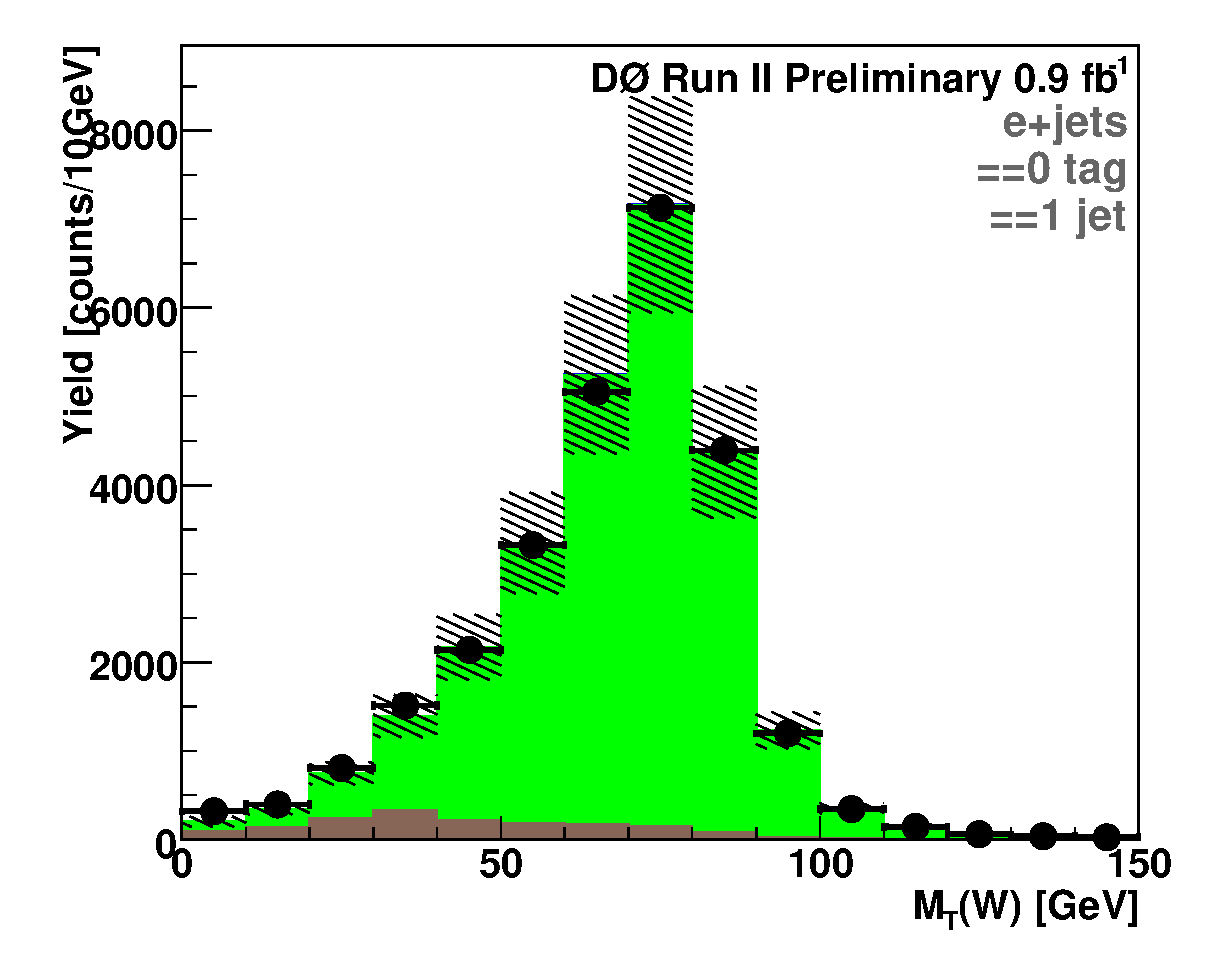
\includegraphics[width=0.32\textwidth]{figures/electron/CC_EqZeroTag_EqOneJet_WTransverseMass.eps}  
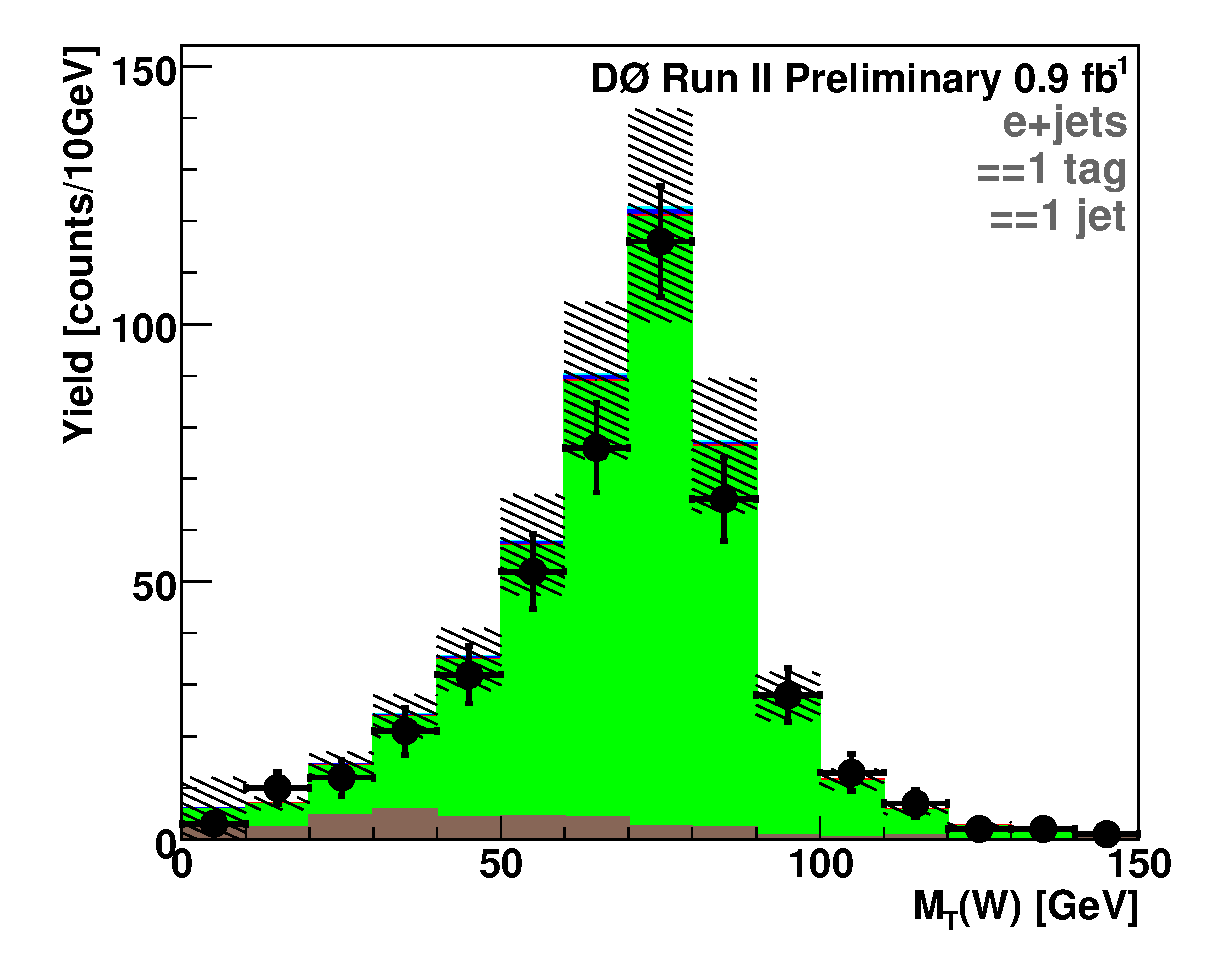
\includegraphics[width=0.32\textwidth]{figures/electron/CC_EqOneTag_EqOneJet_WTransverseMass.eps}   

\includegraphics[width=0.32\textwidth]{figures/electron/WTransverseMass_placeholder.eps}            
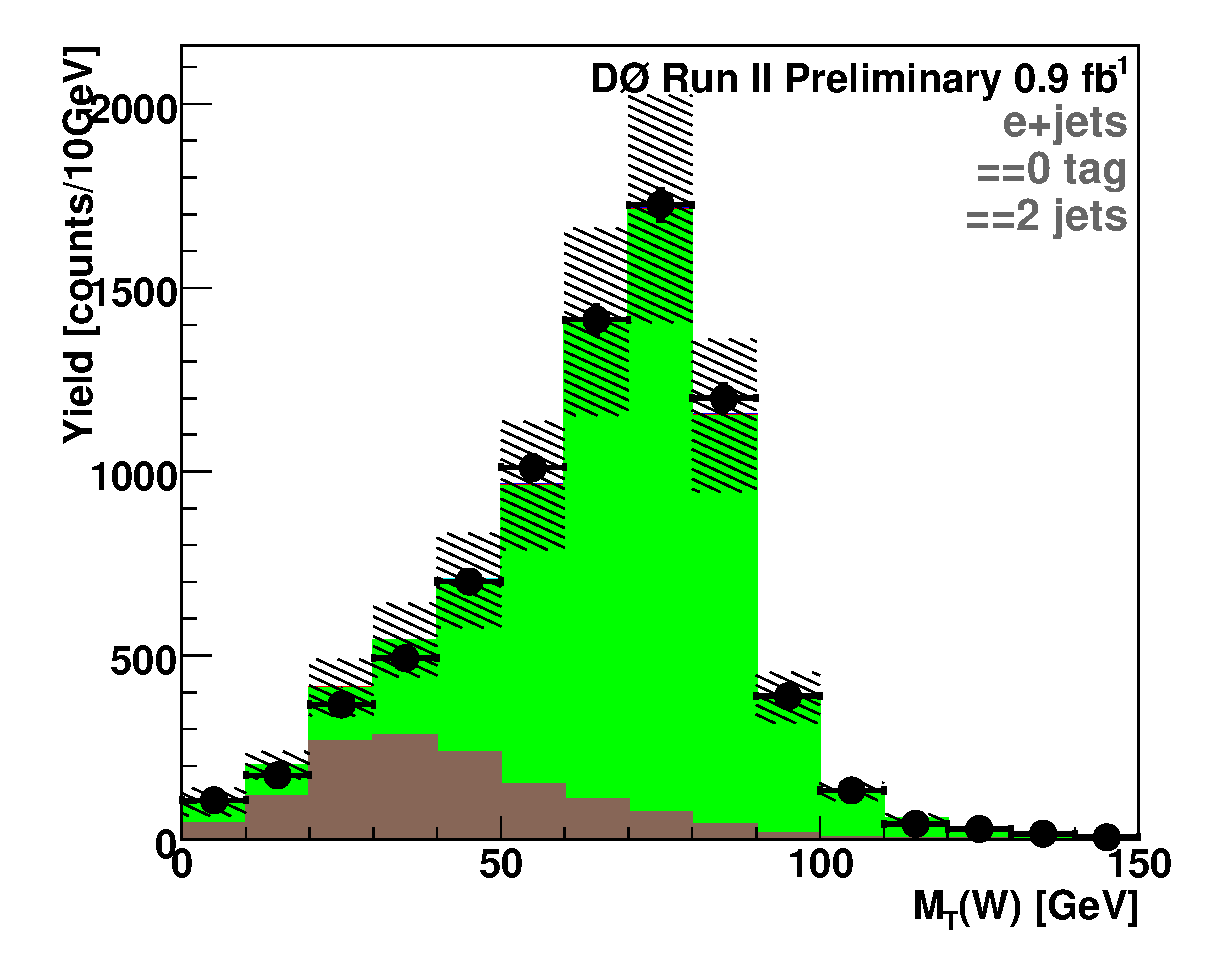
\includegraphics[width=0.32\textwidth]{figures/electron/CC_EqZeroTag_EqTwoJet_WTransverseMass.eps}  
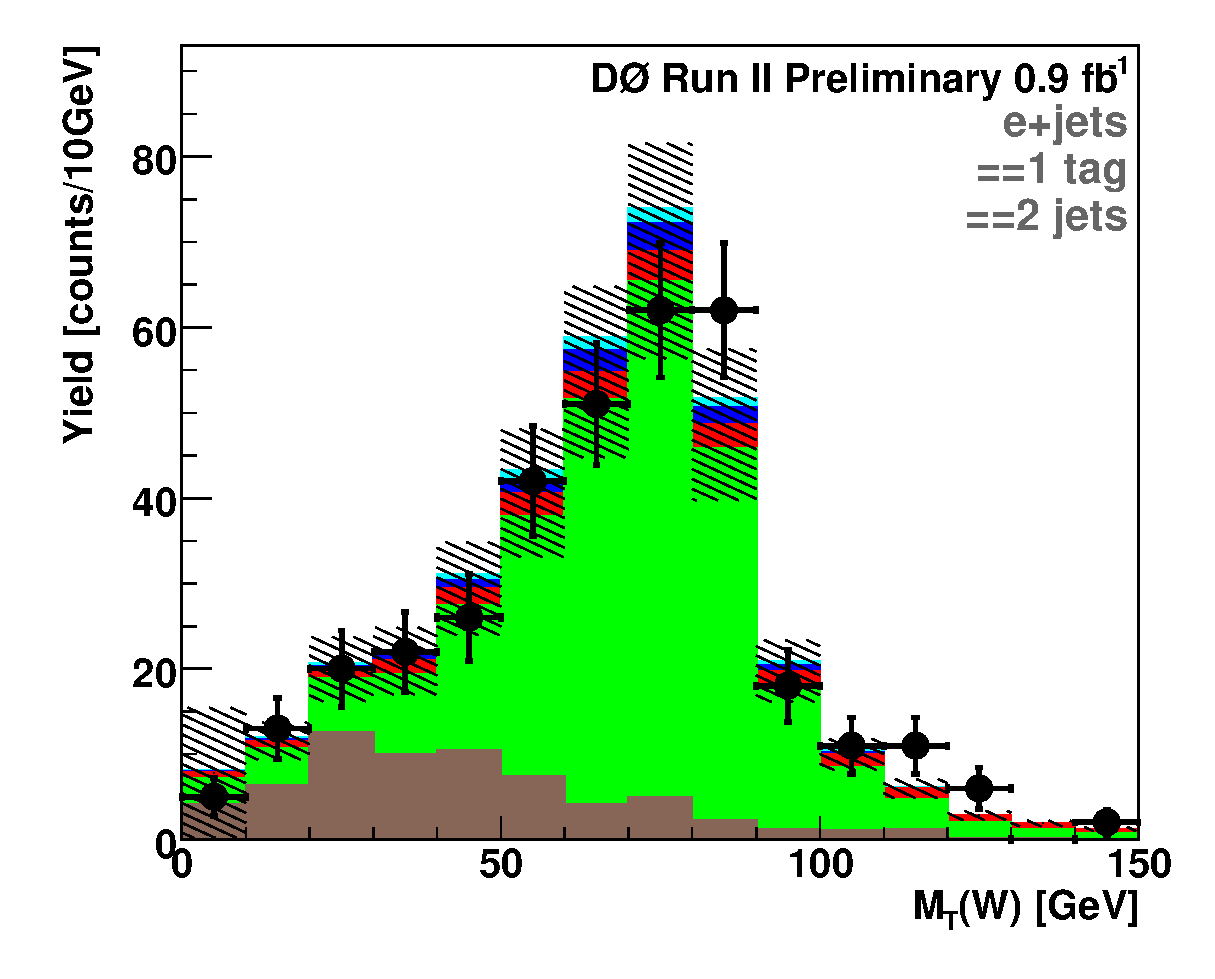
\includegraphics[width=0.32\textwidth]{figures/electron/CC_EqOneTag_EqTwoJet_WTransverseMass.eps}   
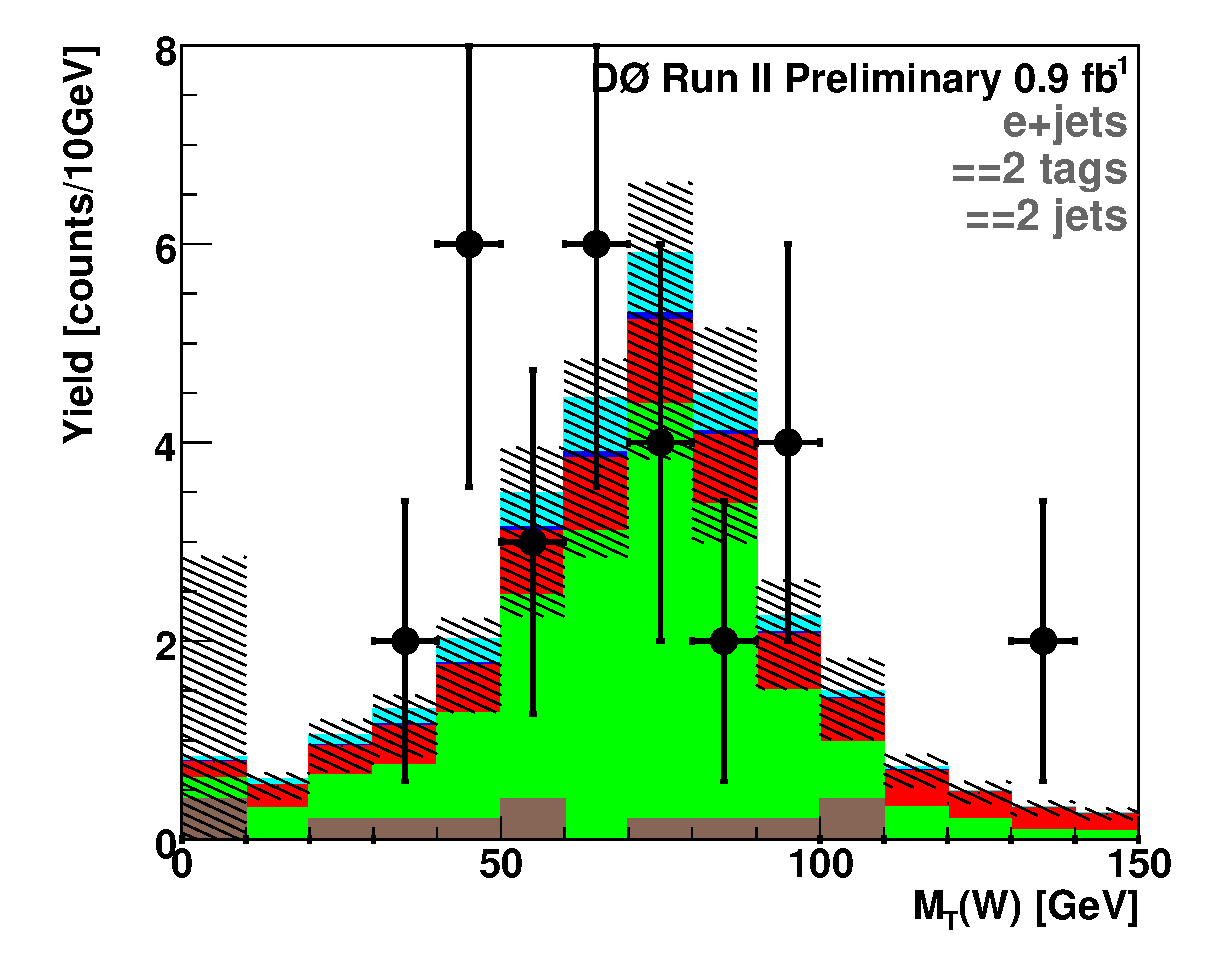
\includegraphics[width=0.32\textwidth]{figures/electron/CC_EqTwoTag_EqTwoJet_WTransverseMass.eps}   
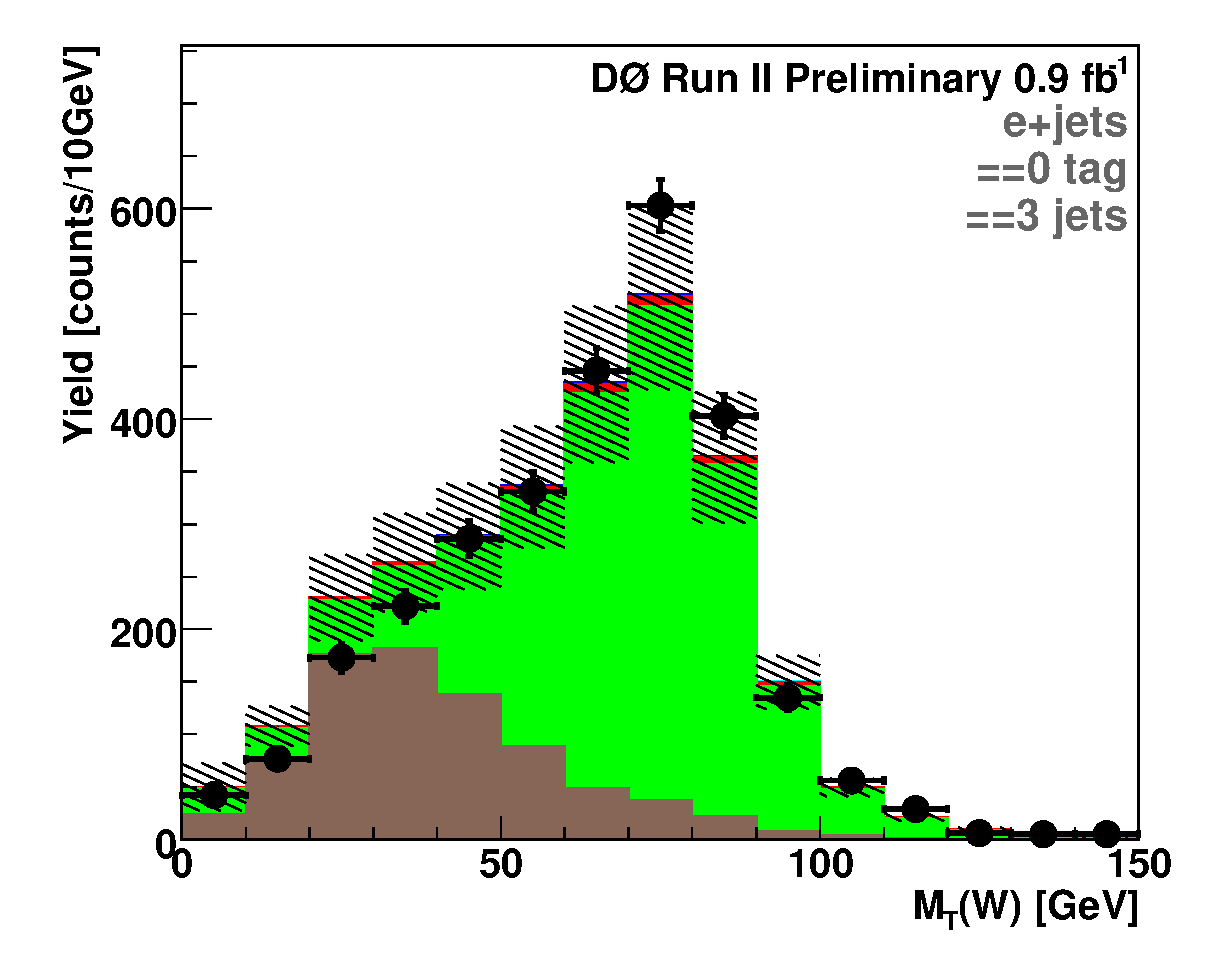
\includegraphics[width=0.32\textwidth]{figures/electron/CC_EqZeroTag_EqThreeJet_WTransverseMass.eps}
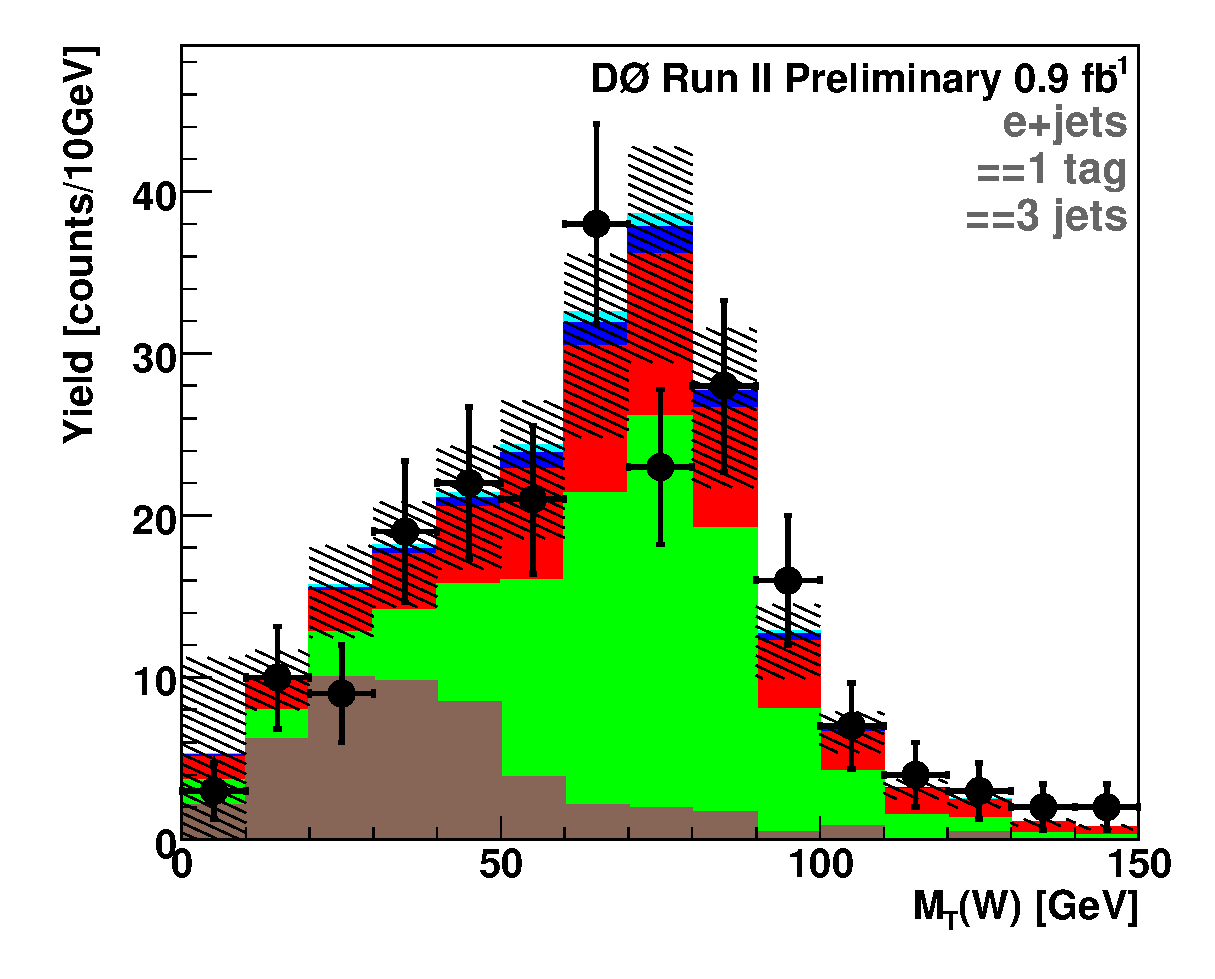
\includegraphics[width=0.32\textwidth]{figures/electron/CC_EqOneTag_EqThreeJet_WTransverseMass.eps} 
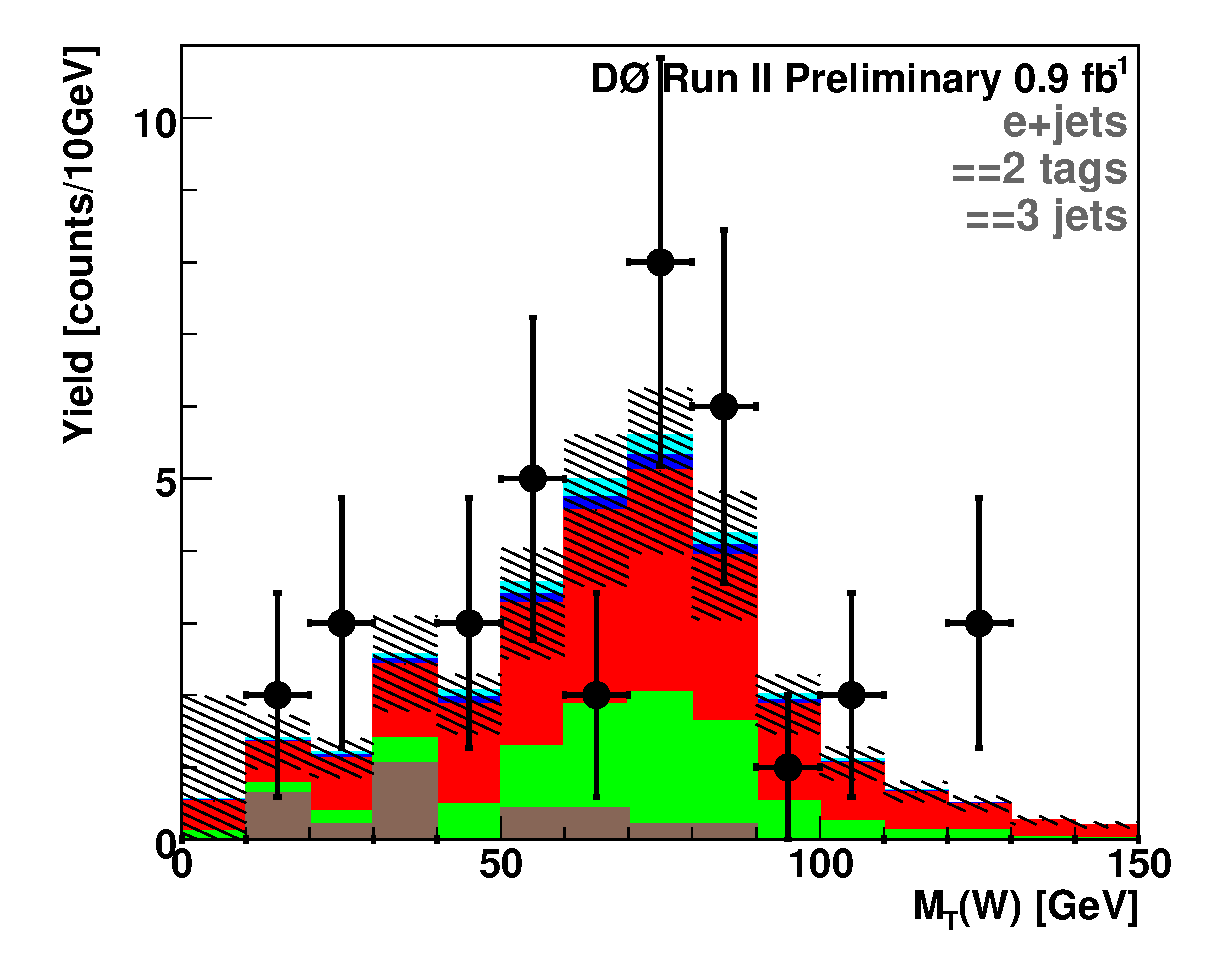
\includegraphics[width=0.32\textwidth]{figures/electron/CC_EqTwoTag_EqThreeJet_WTransverseMass.eps} 
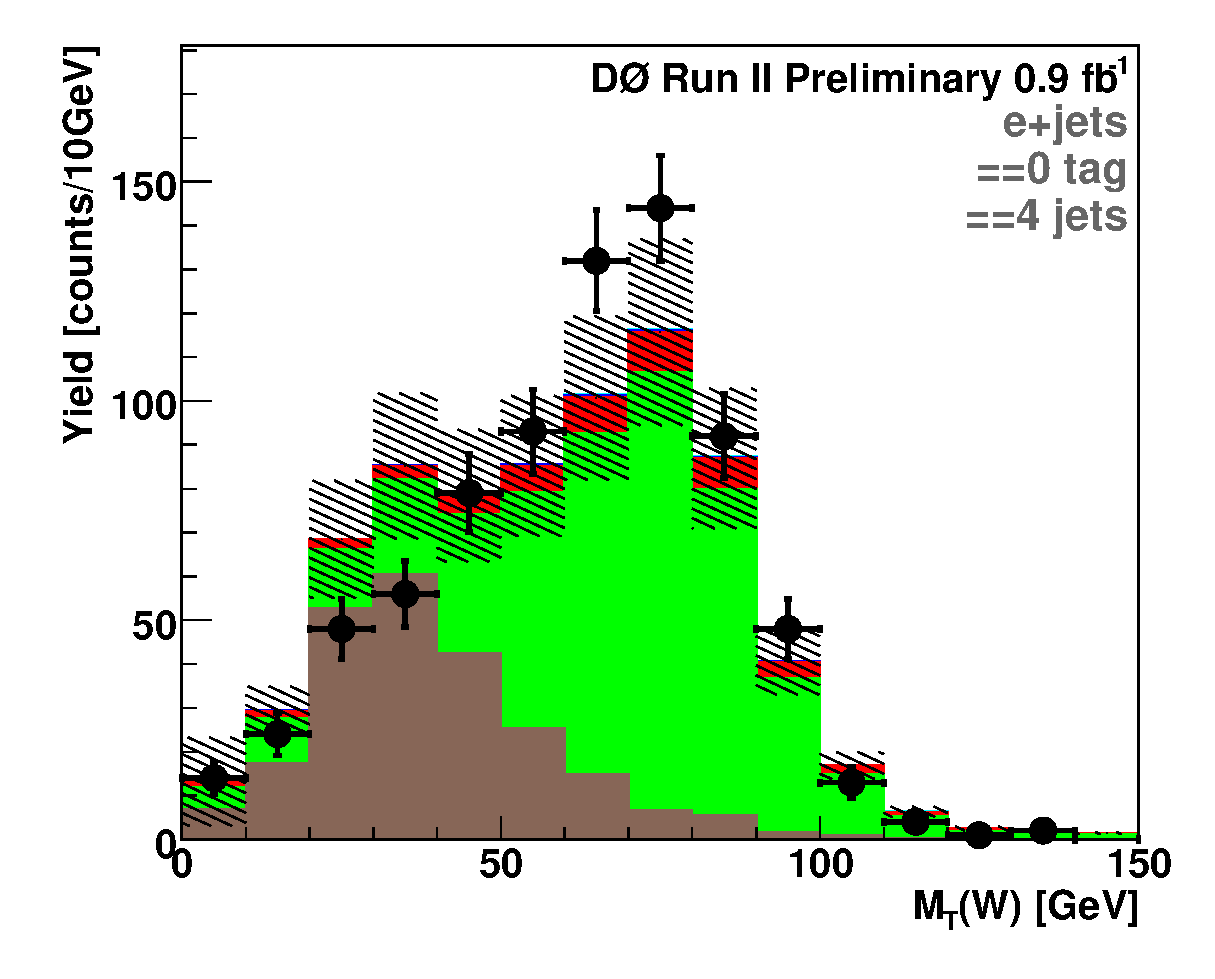
\includegraphics[width=0.32\textwidth]{figures/electron/CC_EqZeroTag_EqFourJet_WTransverseMass.eps} 
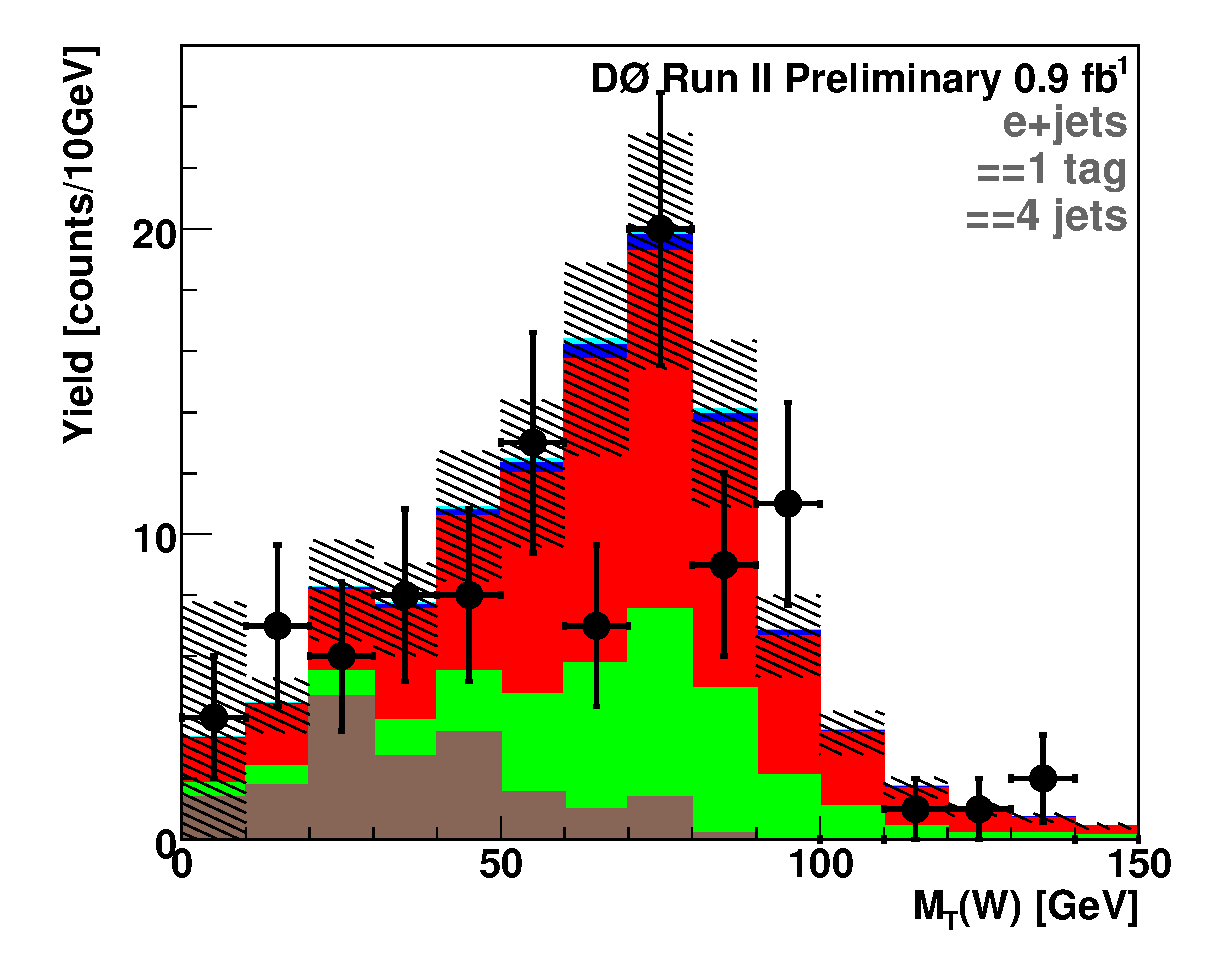
\includegraphics[width=0.32\textwidth]{figures/electron/CC_EqOneTag_EqFourJet_WTransverseMass.eps}  
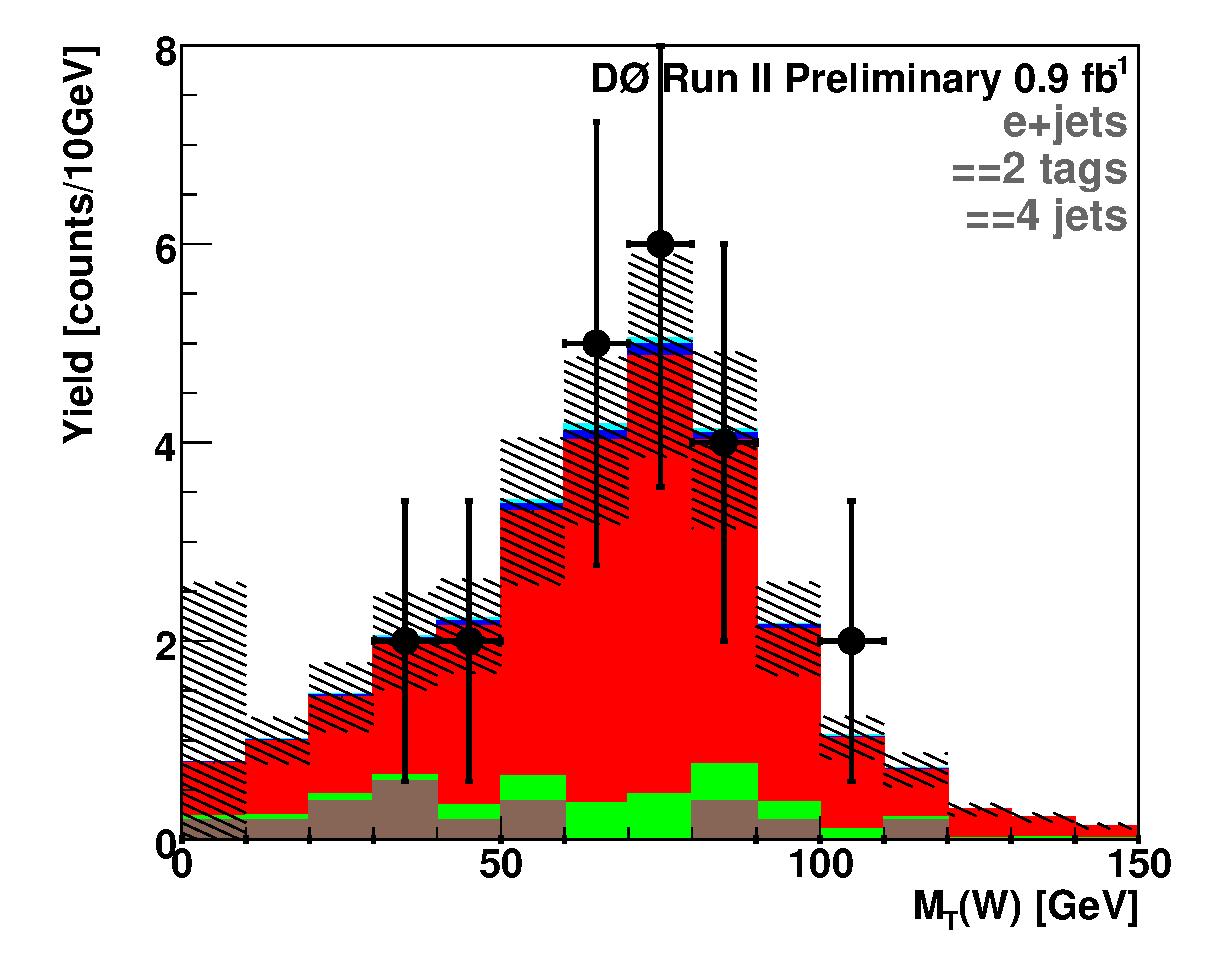
\includegraphics[width=0.32\textwidth]{figures/electron/CC_EqTwoTag_EqFourJet_WTransverseMass.eps}  
\vspace{-0.1in}
\caption[MTWelectron]{The $W$~boson transverse mass distributions for
the electron channel event samples after selection with zero tagged
jets (left column), one tagged jet (middle column), and two tagged
jets (right column). Events in the first row have one jet, in the
second row they have two jets, in the third row, three jets, and in
the fourth row, four jets.}
\label{MTW-electron}
\end{figure}

\clearpage

\begin{center}
W TRANSVERSE MASS IN THE MUON CHANNEL
\end{center}

\begin{figure}[!h!tbp]
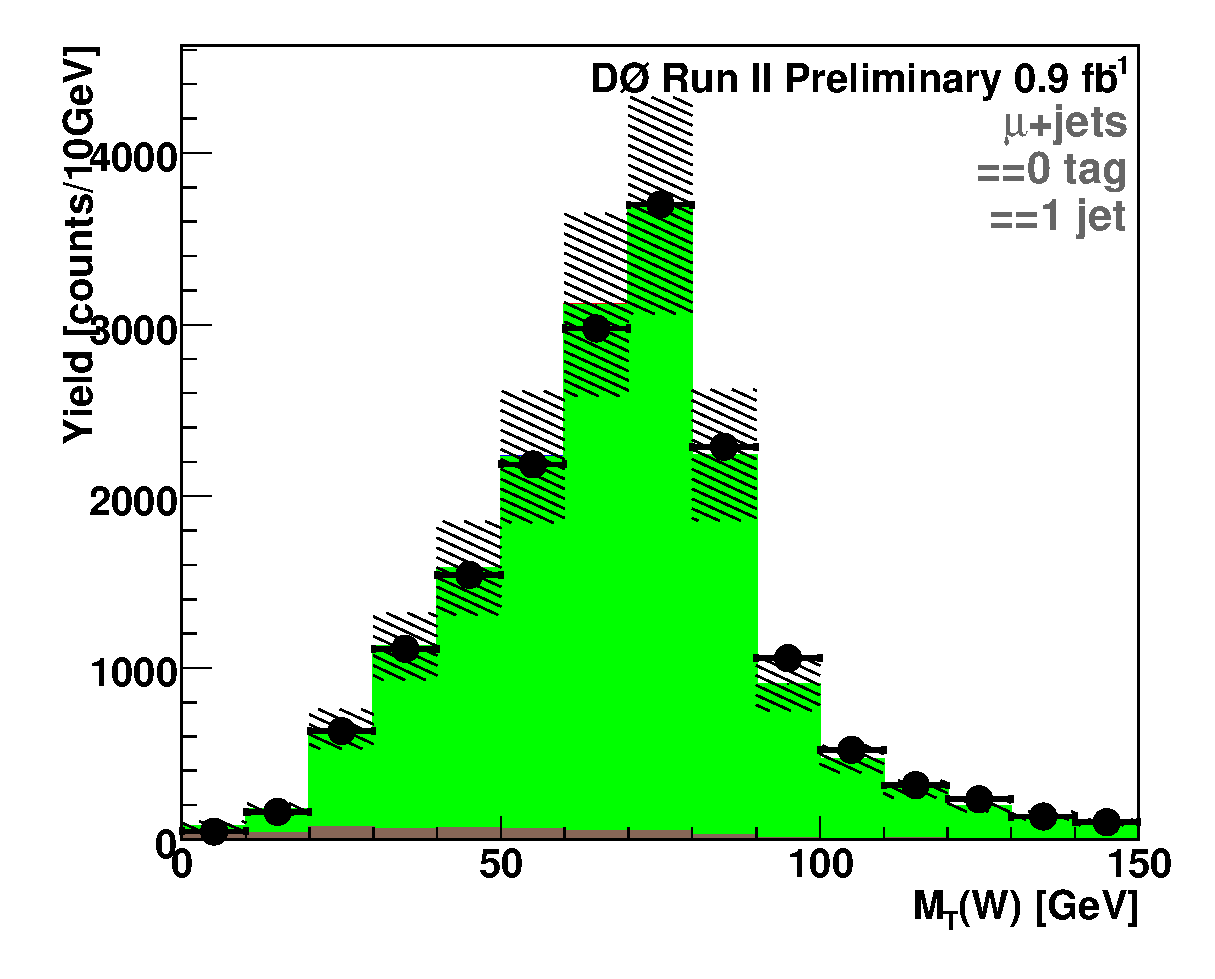
\includegraphics[width=0.32\textwidth]{figures/muon/mu_EqZeroTag_EqOneJet_WTransverseMass.eps}  
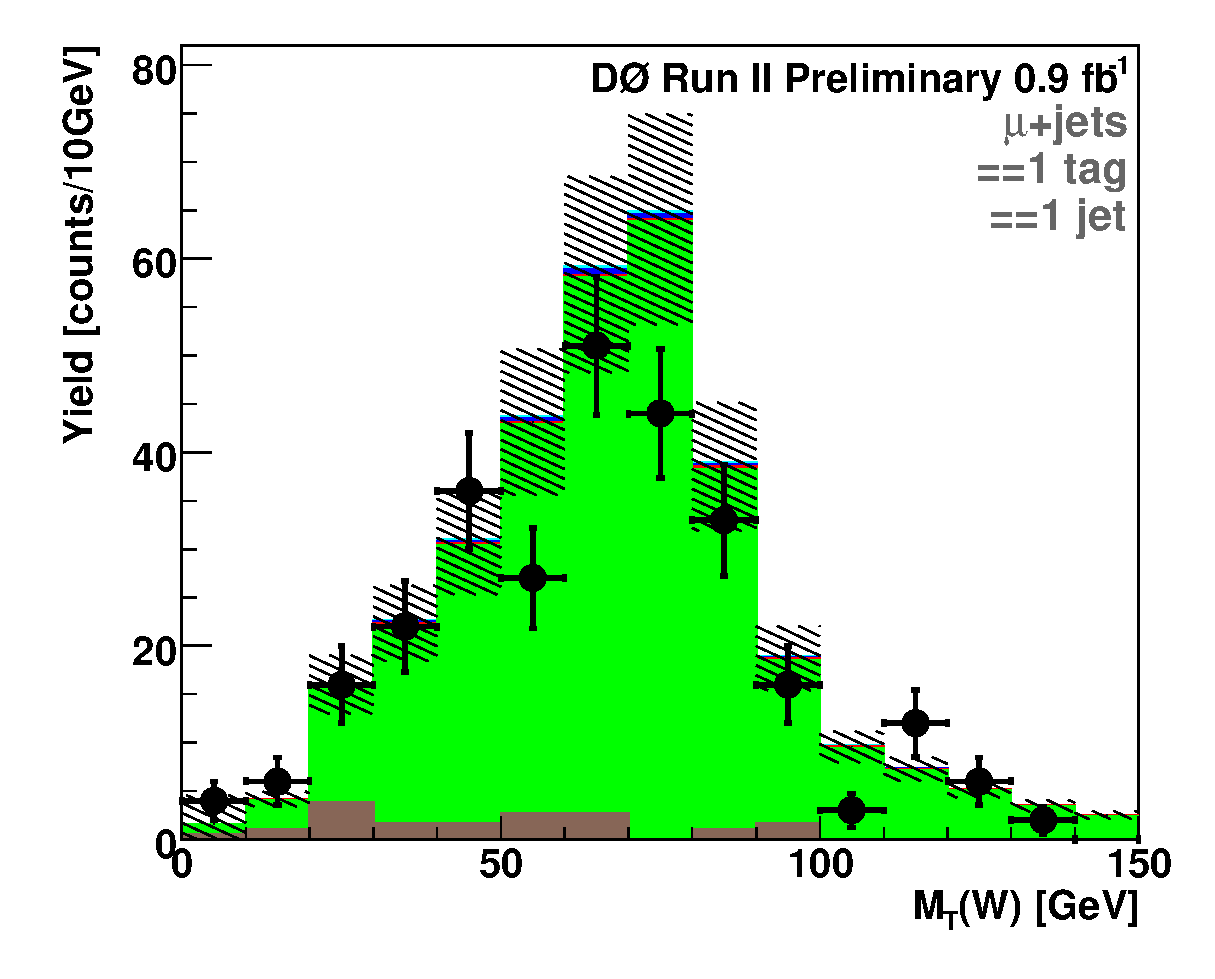
\includegraphics[width=0.32\textwidth]{figures/muon/mu_EqOneTag_EqOneJet_WTransverseMass.eps}   

\includegraphics[width=0.32\textwidth]{figures/muon/WTransverseMass_placeholder.eps}            
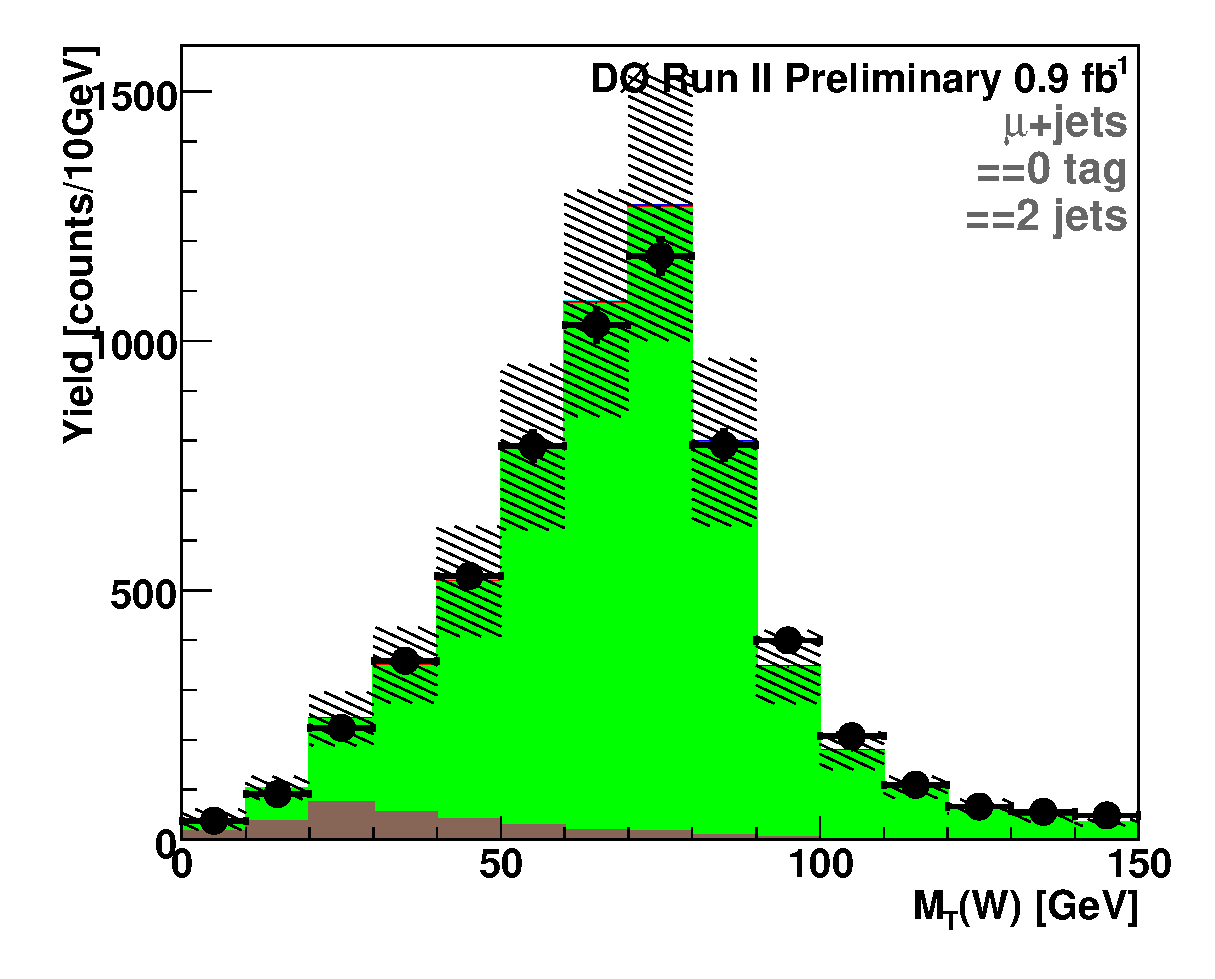
\includegraphics[width=0.32\textwidth]{figures/muon/mu_EqZeroTag_EqTwoJet_WTransverseMass.eps}  
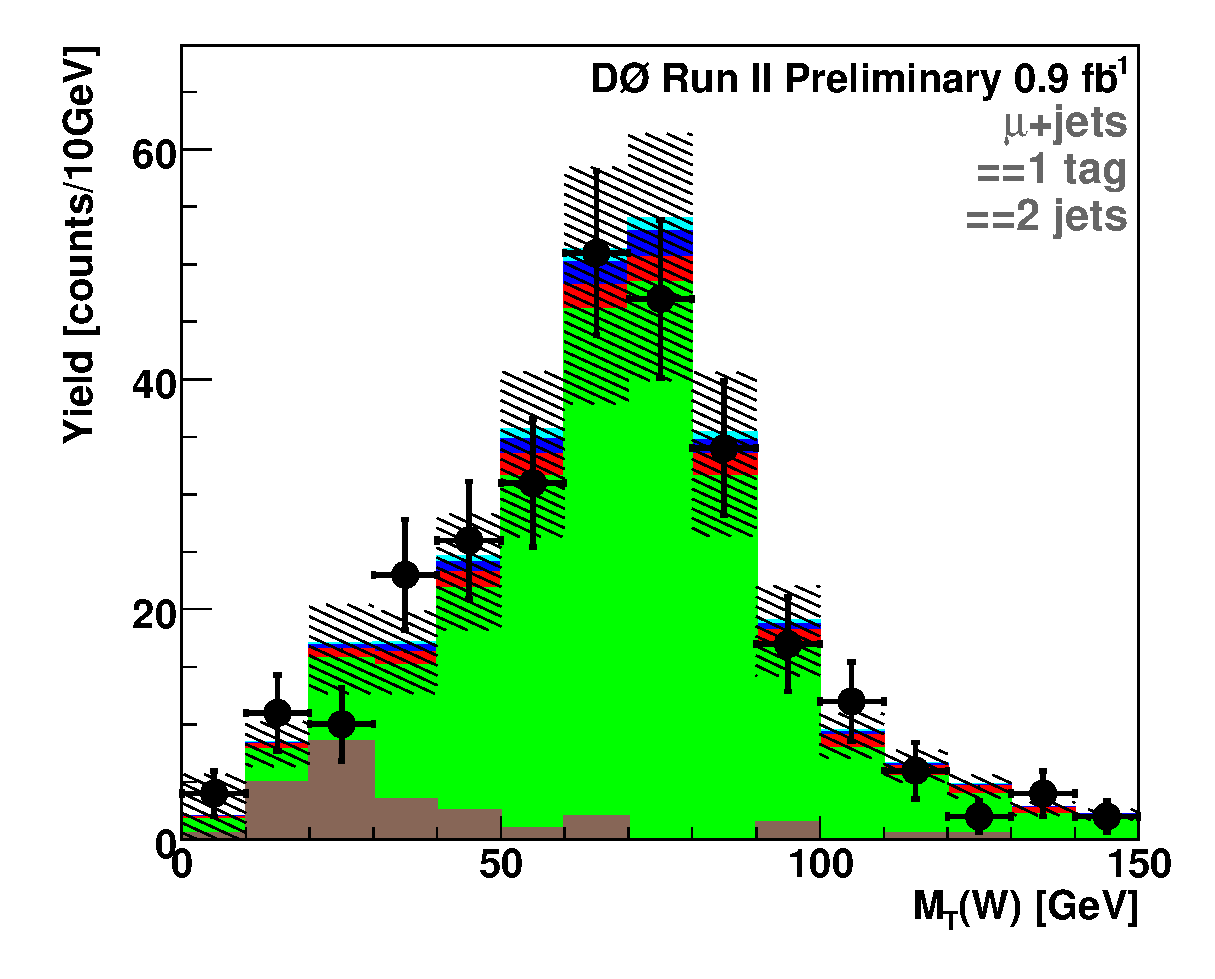
\includegraphics[width=0.32\textwidth]{figures/muon/mu_EqOneTag_EqTwoJet_WTransverseMass.eps}   
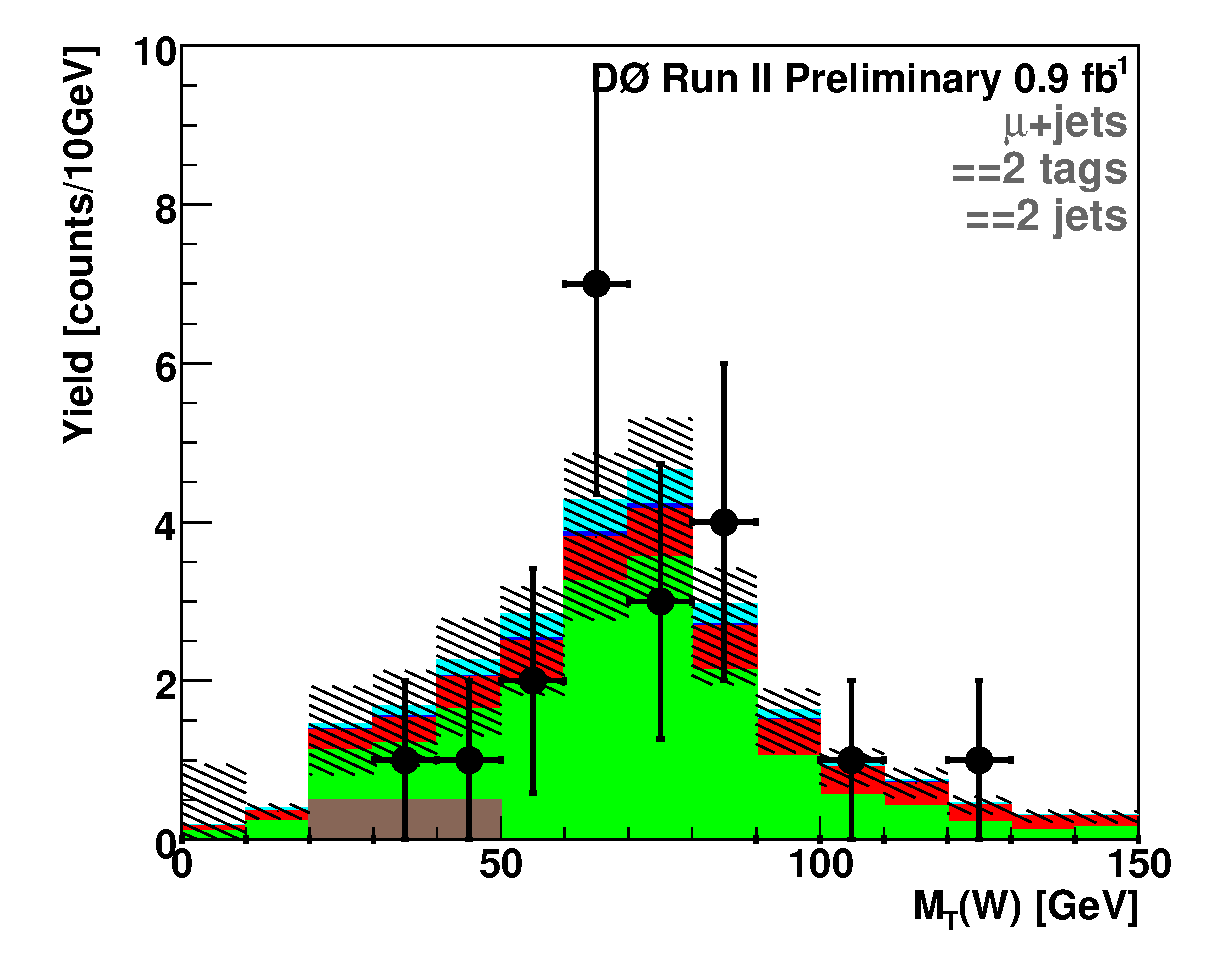
\includegraphics[width=0.32\textwidth]{figures/muon/mu_EqTwoTag_EqTwoJet_WTransverseMass.eps}   
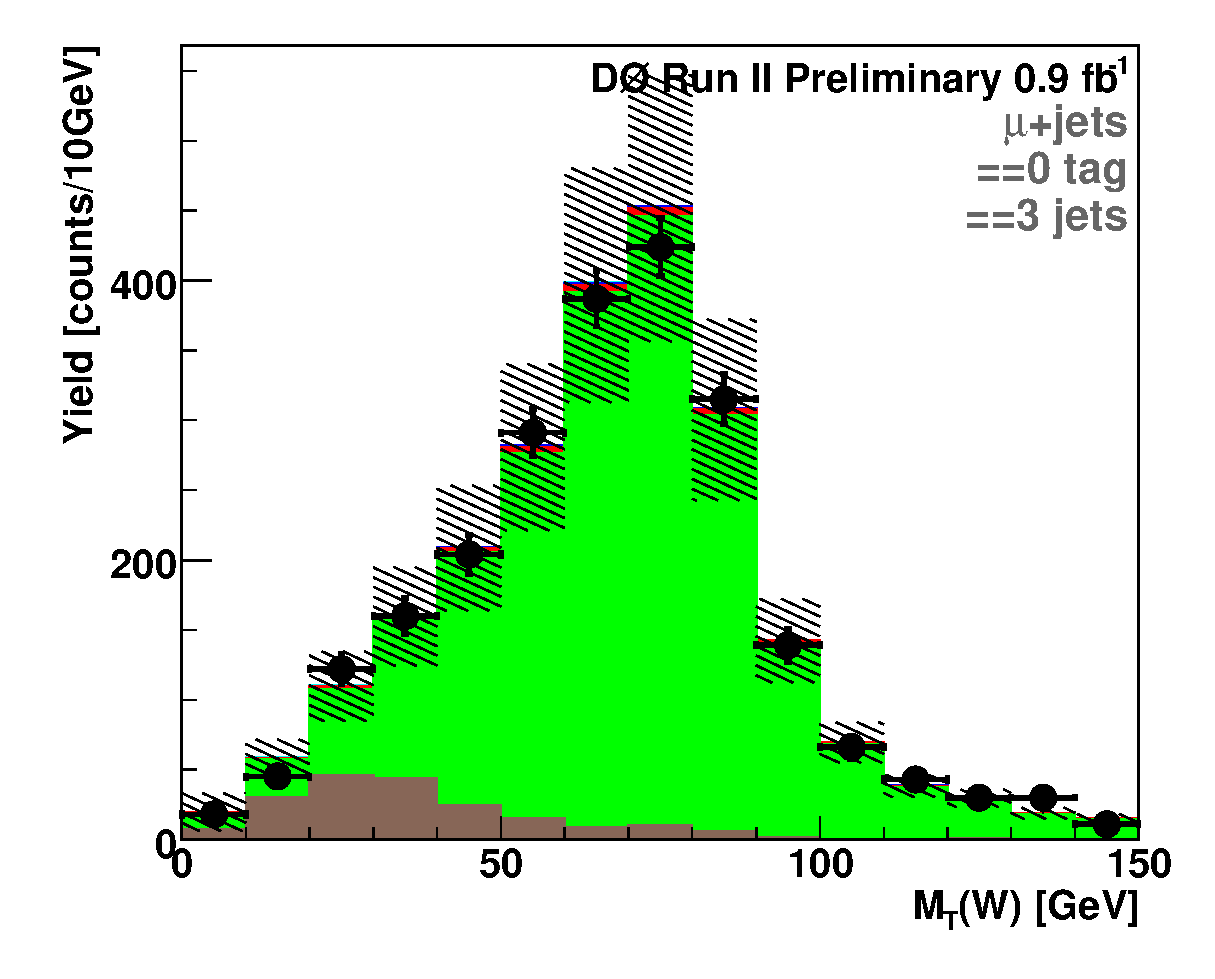
\includegraphics[width=0.32\textwidth]{figures/muon/mu_EqZeroTag_EqThreeJet_WTransverseMass.eps}
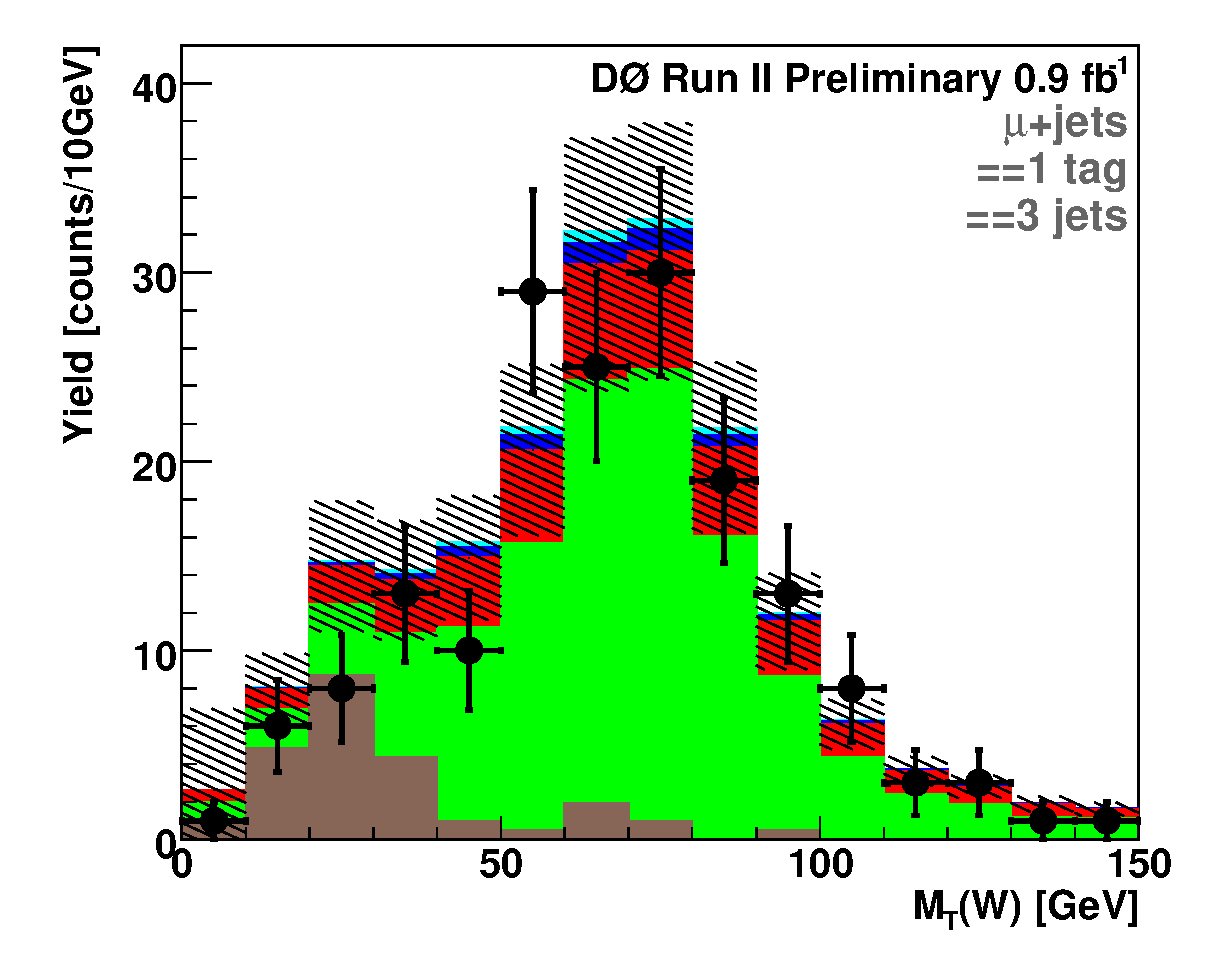
\includegraphics[width=0.32\textwidth]{figures/muon/mu_EqOneTag_EqThreeJet_WTransverseMass.eps} 
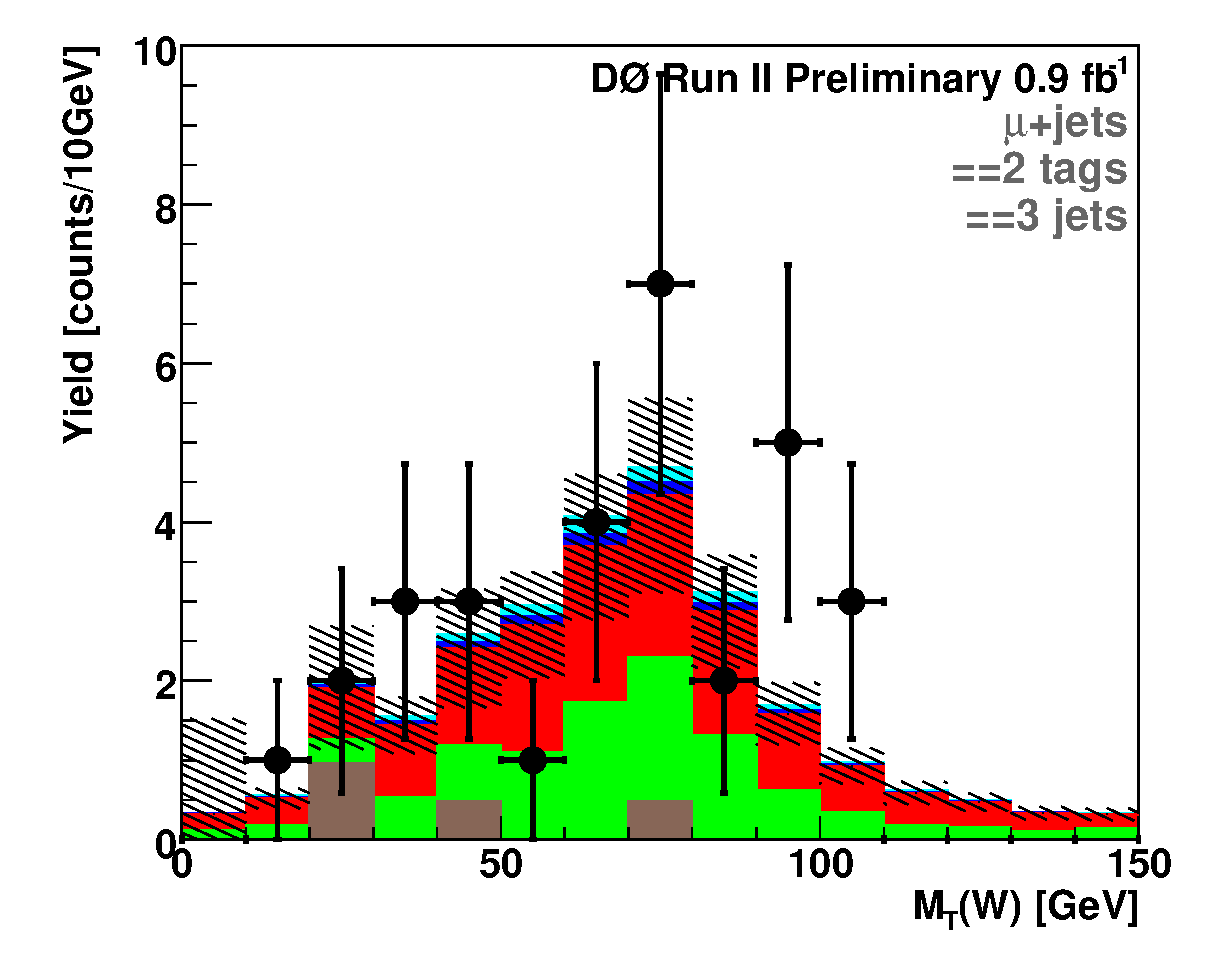
\includegraphics[width=0.32\textwidth]{figures/muon/mu_EqTwoTag_EqThreeJet_WTransverseMass.eps} 
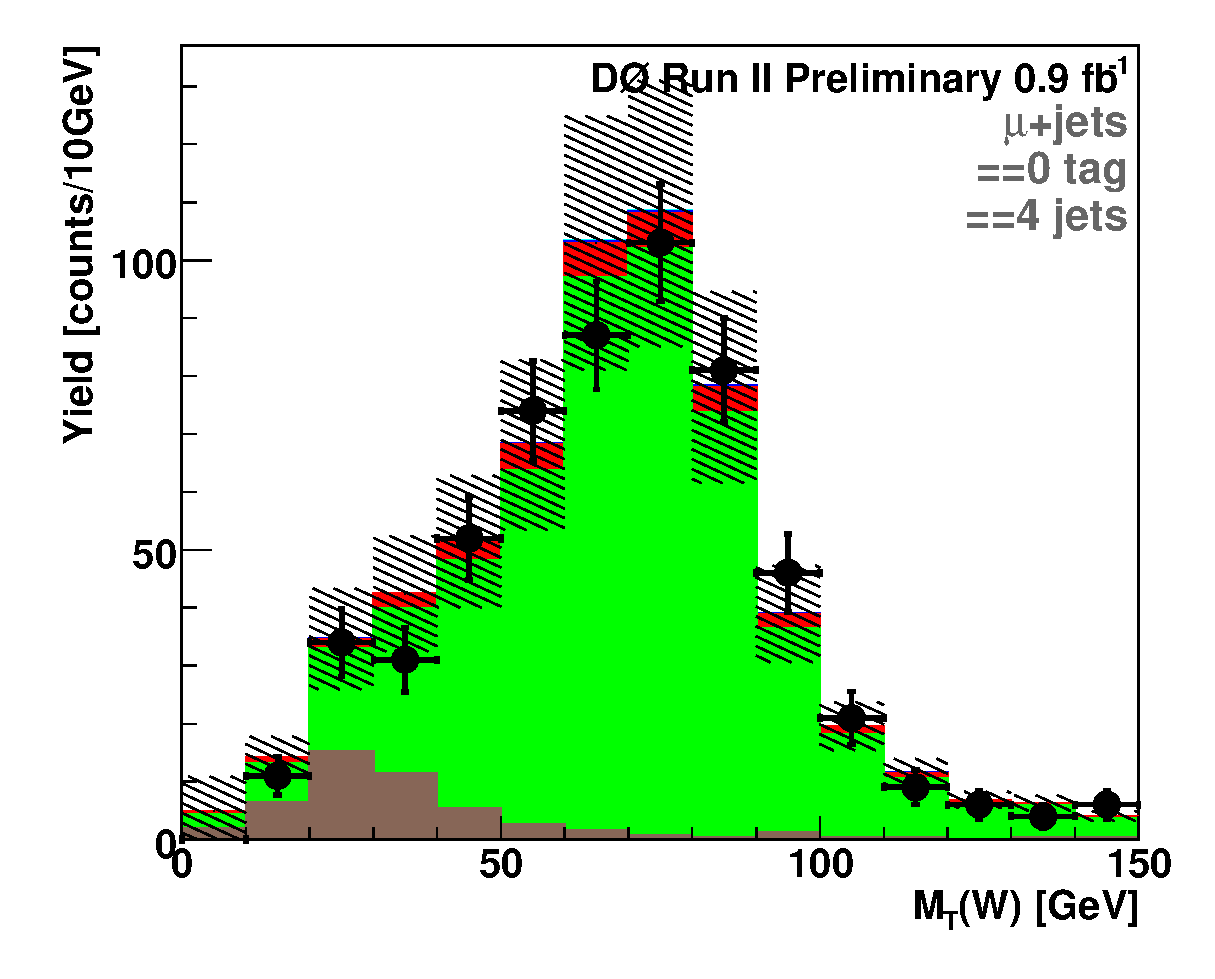
\includegraphics[width=0.32\textwidth]{figures/muon/mu_EqZeroTag_EqFourJet_WTransverseMass.eps} 
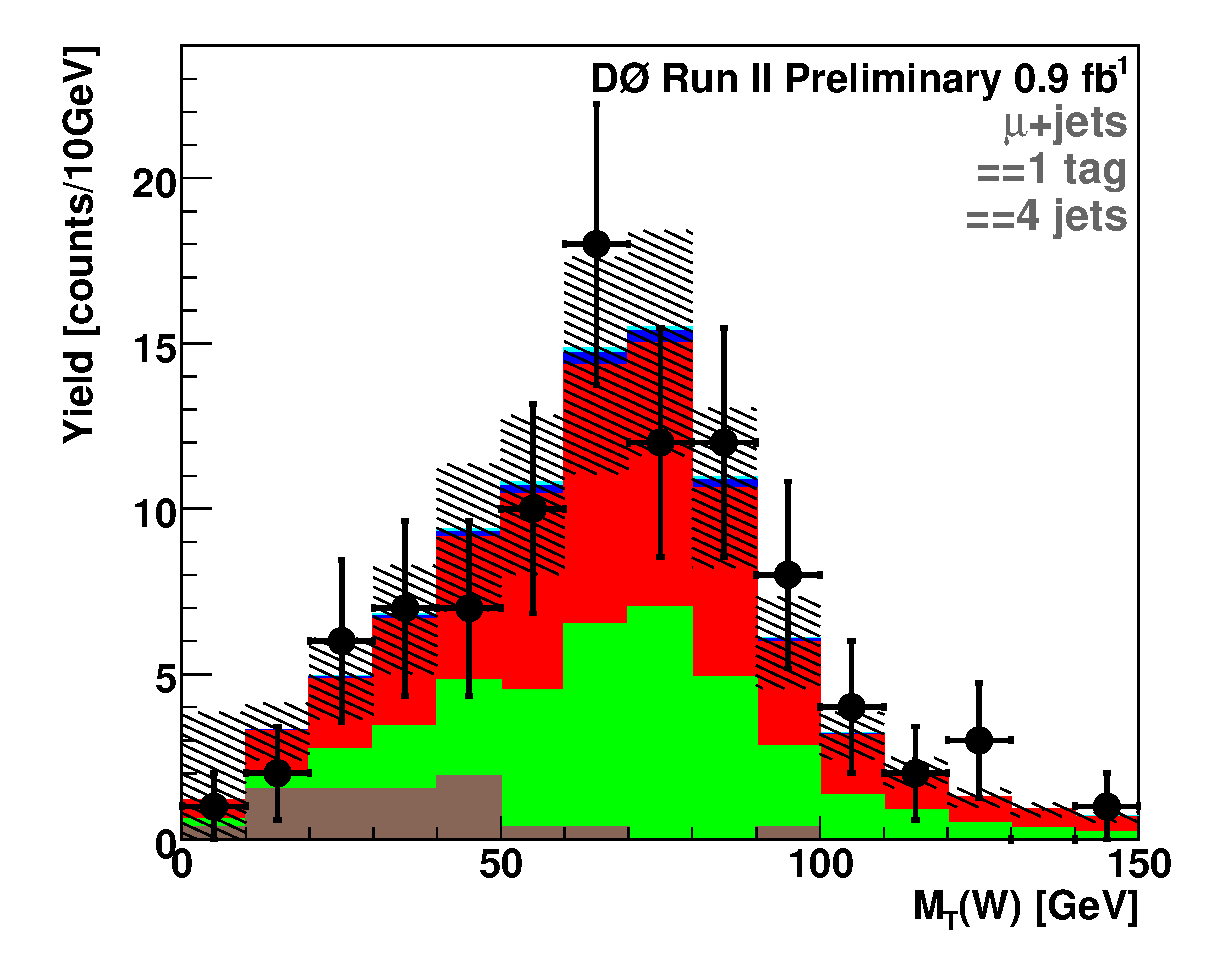
\includegraphics[width=0.32\textwidth]{figures/muon/mu_EqOneTag_EqFourJet_WTransverseMass.eps}  
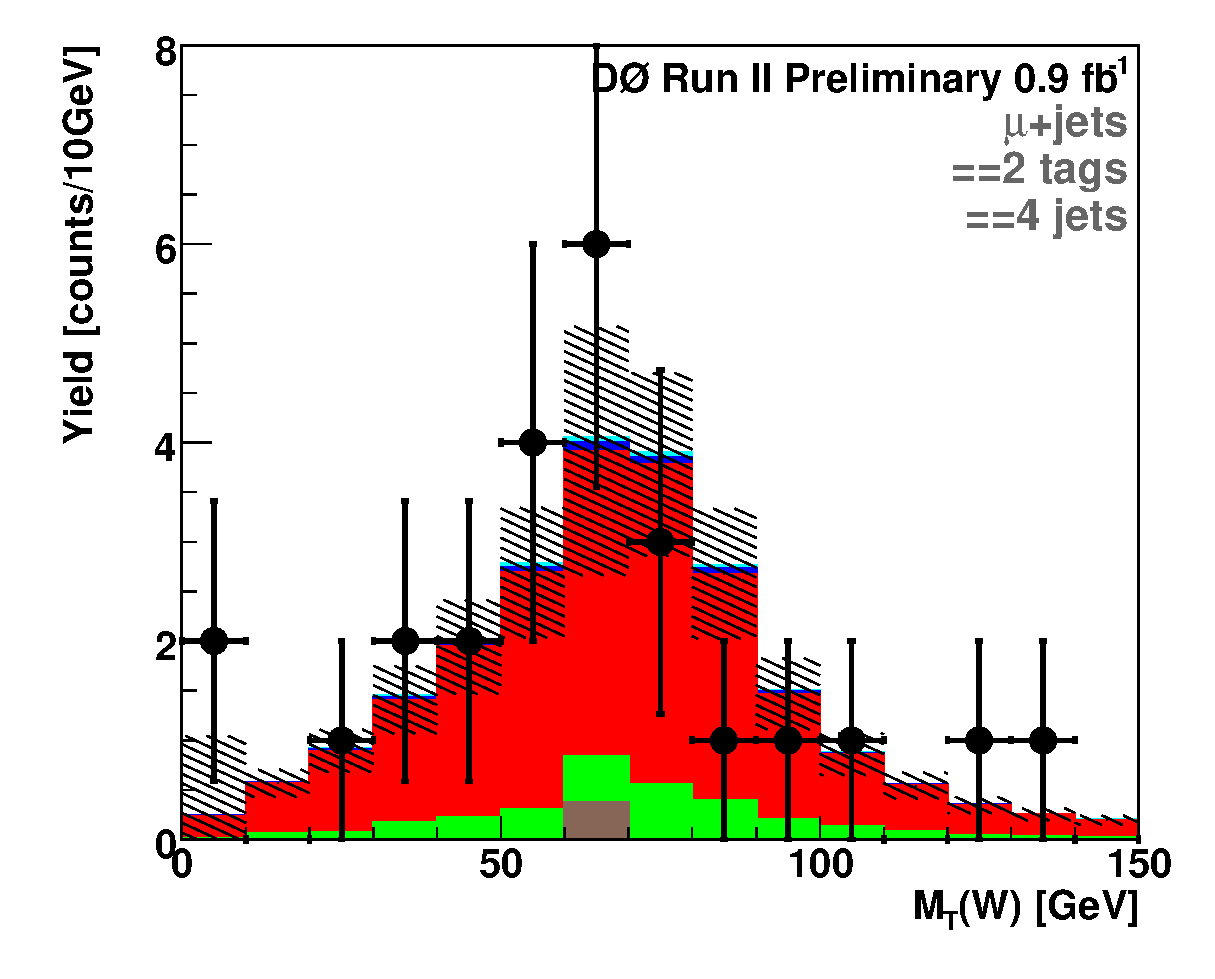
\includegraphics[width=0.32\textwidth]{figures/muon/mu_EqTwoTag_EqFourJet_WTransverseMass.eps}  
\vspace{-0.1in}
\caption[MTWmuon]{The $W$~boson transverse mass distributions for
the muon channel event samples after selection with zero tagged
jets (left column), one tagged jet (middle column), and two tagged
jets (right column). Events in the first row have one jet, in the
second row they have two jets, in the third row, three jets, and in
the forth row, four jets.}
\label{MTW-muon}
\end{figure}
